\documentclass[runningheads,envcountsame]{llncs}



% ORCID
\makeatletter
\RequirePackage[bookmarks,unicode,colorlinks=true]{hyperref}%
   \def\@citecolor{blue}%
   \def\@urlcolor{blue}%
   \def\@linkcolor{blue}%
\def\UrlFont{\rmfamily}
\def\orcidID#1{\href{http://orcid.org/#1}{\protect\raisebox{-1.25pt}{\protect
\includegraphics{orcid_color.eps}}}}
\makeatother


% Since we use the hyperref package, Springer asks us to include the following line
% to display URLs in blue roman font according to Springer's eBook style:
\renewcommand\UrlFont{\color{blue}\rmfamily}


\usepackage{xcolor,colortbl}
\usepackage{mathtools}
\usepackage{multirow}
\usepackage{stmaryrd}
\usepackage{cancel}
\usepackage{amsmath,amssymb}
\usepackage{thmtools, thm-restate}
\usepackage[shortlabels]{enumitem}
\usepackage{microtype}
\usepackage{wrapfig}
\usepackage{pbox}
\usepackage{marvosym}
\usepackage{listings}
\usepackage[ruled, vlined, linesnumbered]{algorithm2e}
\hypersetup{
	pdftitle={A Dependency Pair Framework for Relative Termination of Term Rewriting}, colorlinks=true, linkcolor=blue, citecolor=olive, filecolor=magenta, urlcolor=cyan
}
\usepackage{todonotes}
\usepackage{placeins}
\usepackage{float}
\usepackage{tikz}
\usepackage{caption}
\usepackage{subcaption}
\usepackage{mymatrix}
\usepackage{nicefrac,xfrac}
\usetikzlibrary{shapes,calc,arrows,automata,decorations.pathmorphing,backgrounds}
\usepackage[all,cmtip]{xy}

\RequirePackage{makecell}

\usepackage[capitalize,nameinlink]{cleveref}
\usepackage{IEEEtrantools}
\renewenvironment{proof}{}{}
\newenvironment{myproof}{
	\noindent{\it Proof.}
}{\qed
	\medskip
}
%%%%%%%%%%%%%%%%%%%%%%%%%%%%% USER-DEFINED MACROS %%%%%%%%%%%%%%%%%%%%%%%%%%%%%
\def\namedlabel#1#2{\begingroup
    #2%
    \def\@currentlabel{#2}%
    \phantomsection\label{#1}\endgroup
}

%\newcommand{\comment}[1]{\footnote{!!!#1}}
%\renewcommand{\comment}[1]{}
%\newcommand{\disabledcomment}[1]{}
%\newcommand{\oldcomment}[1]{}

%% Operators
\newcommand{\diff}{\mathop{}\!\mathrm{d}}
\renewcommand{\Re}{\operatorname{Re}}
\renewcommand{\Im}{\operatorname{Im}}
\DeclareMathOperator{\im}{im}
\DeclareMathOperator{\rank}{rank}

%% Bold face
\newcommand{\ba}{\mathbf{a}}
\newcommand{\bb}{\mathbf{b}}
\newcommand{\bx}{\mathbf{x}}
\newcommand{\by}{\mathbf{y}}
\newcommand{\bzero}{\mathbf{0}}
\newcommand{\bone}{\mathbf{1}}

%% Miscellaneous
\newcommand{\ie}{\leavevmode\unskip, i.e.,\xspace}
\newcommand{\eg}{\leavevmode\unskip, e.g.,\xspace}
\newcommand{\dash}{\textthreequartersemdash\xspace}
\newcommand{\TikZ}{Ti\textit{k}Z\xspace}
\newcommand{\matlab}{\textsc{Matlab}\xspace}
\newcommand{\aprove}{\textsf{AProVE}}
\newcommand{\muterm}{\textsf{MU-TERM}}
\newcommand{\natt}{\textsf{NaTT}}
\newcommand{\ttttwo}{\textsf{T\kern-0.15em\raisebox{-0.55ex}T\kern-0.15emT\kern-0.15em\raisebox{-0.55ex}2}}
\newcommand{\ceta}{\textsf{CeTA}}
\newcommand{\mnm}{\textsf{MultumNonMulta}}
\newcommand{\matchbox}{\textsf{Matchbox}}

\newcounter{saveenum}
\newcommand{\name}[1]{\textsc{#1}}
\renewcommand{\emph}[1]{\index{#1}\textit{#1}}
\newcommand{\bref}[1]{(\ref{#1})}

%% General Math
\renewcommand{\emptyset}{\varnothing}
\newcommand{\dashed}[1]{#1^{\prime}}
\newcommand{\IB}{\mathbb{B}}
\newcommand{\IP}{\mathbb{P}}
\newcommand{\IZ}{\mathbb{Z}}
\newcommand{\IN}{\mathbb{N}}
\newcommand{\IR}{\mathbb{R}}
\newcommand{\expec}[1]{\ensuremath{\mathbb{E}\left(#1\right)}}
\newcommand{\IE}{\ensuremath{\mathbb{E}}}
\newcommand{\II}{\mathbb{I}}
\newcommand{\F}[1]{\mathfrak{#1}}
\newcommand{\C}[1]{\mathcal{#1}}
\newcommand{\sigmagen}[1]{\ensuremath{\left\langle #1 \right \rangle _{\sigma}}}
\newcommand{\multiset}[1]{\mathrm{MultiSet}(#1)}
\newcommand{\pot}[1]{\mathrm{Pot}(#1)}
\newcommand{\mymap}[2]{\mathrm{Map}(#1,#2)}
\newcommand{\ind}{\mathbf{1}}

\newcommand{\leftleadsto}{\mathrel{\reflectbox{$\leadsto$}}}

%% Termrewriting 
\makeatletter
\def\moverlay{\mathpalette\mov@rlay}
\def\mov@rlay#1#2{\leavevmode\vtop{%
   \baselineskip\z@skip \lineskiplimit-\maxdimen
   \ialign{\hfil$\m@th#1##$\hfil\cr#2\crcr}}}
\newcommand{\charfusion}[3][\mathord]{
    #1{\ifx#1\mathop\vphantom{#2}\fi
        \mathpalette\mov@rlay{#2\cr#3}
      }
    \ifx#1\mathop\expandafter\displaylimits\fi}
\makeatother

%%% General Definitions
\newcommand{\Var}{\mathcal{V}}
\newcommand{\Loc}{\mathcal{L}}
\newcommand{\Trans}{\mathcal{T}}
\renewcommand{\P}{\mathcal{P}}
\newcommand{\eval}{\sigma}
\newcommand{\occ}{\operatorname{Occ}}
\newcommand{\redexocc}{\operatorname{pirp}}
\newcommand{\varocc}{\operatorname{Occ}_{\C{V}}}

%%% PTRS and DP Stuff
\newcommand{\Proc}{\operatorname{Proc}}
\newcommand{\projOne}{\mathrm{proj}_1}
\newcommand{\projTwo}{\mathrm{proj}_2}
\newcommand{\MSubd}{\mathrm{MSub}_D}
\newcommand{\Subd}{\mathrm{Sub}_D}
\newcommand{\SubdPos}{\mathrm{Sub}_{DPos}}
\newcommand{\SubdOcc}{\mathrm{Sub}_{DOcc}}
\newcommand{\SubdSharp}{\mathrm{Sub}^\#}
\newcommand{\SubdPosSharp}{\mathrm{Sub}_{DPos}^\#}
\newcommand{\SubdR}{\mathrm{Sub}_{D, \R}^\#}
\newcommand{\SubdD}{\mathrm{Sub}_{D, \C{D}}^\#}
\newcommand{\SubdSharpNotNorm}{\mathrm{Sub}_{D, \lnot \mathit{nf}}^\#}
\newcommand{\SubdSharpNorm}{\mathrm{Sub}_{D, \mathit{nf}}^\#}
\newcommand{\Subdnf}{\mathrm{Sub}_D^{\neg \mathit{nf}}}
\newcommand{\Subcomnf}{\mathrm{Sub}_{\Com{}}^{\neg \mathit{nf}}}
\newcommand{\Submultnf}{\mathrm{Sub}_{\text{set}}^{\neg \mathit{nf}}}
\newcommand{\SubdnfAll}{\mathrm{SubAll}_D^{\neg \mathit{nf}}}
\newcommand{\SubcomnfAll}{\mathrm{SubAll}_{\Com{}}^{\neg \mathit{nf}}}
\newcommand{\SubmultnfAll}{\mathrm{SubAll}_{\text{mul}}}
\newcommand{\SubmultD}{\mathrm{Sub}_{D, \text{set}}}
\newcommand{\Subterm}[1]{\mathrm{Subterm}(#1)}
\newcommand{\Subtermdep}[1]{\mathrm{Subterm}_{dep}(#1)}
\newcommand{\SubmultPoss}{\mathrm{Sub}_{\text{set}}^{\text{Poss}}}
\newcommand{\SubDPoss}{\mathrm{Sub}_{\text{term}}^{\text{Poss}}}
\newcommand{\SubmultMain}{\mathrm{Sub}_{\text{set}}^{\text{Main}}}
\newcommand{\SubDMain}{\mathrm{Sub}_{\text{term}}^{\text{Main}}}
\newcommand{\SubmultNorm}{\mathrm{Sub}_{\text{set}}^{\text{Norm}}}
\newcommand{\SubDNorm}{\mathrm{Sub}_{\text{term}}^{\text{Norm}}}
\newcommand{\Junk}{\mathrm{Junk}}
\newcommand{\inSet}[1]{\langle \hspace{-3px} \{#1\} \hspace{-3px} \rangle}
\newcommand{\ce}{\mathcal{C}_{\varepsilon}}

\newcommand{\Extension}{\operatorname{Ext}}
\newcommand{\FExtension}{\operatorname{FamExt}}

\newcommand{\Substi}{\operatorname{Sub}}
\newcommand{\SubstitutionSet}[2]{\Substi\left(#1,#2\right)}
\newcommand{\TSet}[2]{\mathcal{T}\left(#1,#2\right)}
\newcommand{\DEPTerm}{\mathcal{T}^\#\left(\Sigma\right)}
\newcommand{\LSet}{\mathcal{L}}
\newcommand{\VSet}{\mathcal{V}}
\newcommand{\TVSet}{\mathcal{TV}}
\newcommand{\PVSet}{\mathcal{PV}}
\newcommand{\DEPSetWellPos}{\mathsf{WPS}}
\newcommand{\PosEx}{\mathsf{PosEx}}
\renewcommand{\O}{\mathcal{O}}
\newcommand{\R}{\mathcal{R}}
\newcommand{\B}{\mathcal{B}}
\newcommand{\pars}[1]{\xrightarrow{p}_{#1}}
\newcommand\restrict[2]{#1\raisebox{-.5ex}{$|$}_{#2}}
\newcommand{\DTuple}[1]{\mathcal{DT}(#1)}
\newcommand{\DPTuple}[1]{\mathcal{DT}_{\!\!pos}(#1)}
\newcommand{\DPair}[1]{\mathcal{DP}(#1)}
\newcommand{\DTPair}[2]{\mathcal{DP}^{#1}(#2)}
\newcommand{\DP}[1]{\mathtt{DP}(#1)}
\newcommand{\Rule}[1]{\mathtt{rule}(#1)}
\newcommand{\ADPair}[2]{\mathcal{A}_{#1}(#2)}
\newcommand{\ADPairMain}[1]{\mathcal{A}_{1}(#1)}
\newcommand{\ADPairBase}[1]{\mathcal{A}_{2}(#1)}
\newcommand{\Dist}{\operatorname{Dist}}
\newcommand{\FDist}{\operatorname{FDist}}
\newcommand{\Supp}{\operatorname{Supp}}
\newcommand{\Hist}{\operatorname{Hist}}
\newcommand{\Term}{\operatorname{Term}}
\newcommand{\NonTerm}{\operatorname{NonTerm}}
\newcommand{\toppos}{\operatorname{\mathcal{T}op}}
\newcommand{\rootsym}{\operatorname{root}}
\newcommand{\capterm}{\operatorname{Cap}}
\newcommand{\renterm}{\operatorname{Ren}}
\newcommand{\rules}{\operatorname{Rules}}
\newcommand{\urules}{\mathcal{U}}
\newcommand{\upairs}{\mathcal{U}\!\text{P}}
\newcommand{\upairsabs}{\mathcal{A}\mathcal{U}\mathcal{P}}
\newcommand{\vr}{\operatorname{vr}}
\newcommand{\capt}{\operatorname{capt}}

\newcommand{\edh}{\operatorname{edh}}
\newcommand{\edl}{\operatorname{edl}}
\newcommand{\Pol}{\operatorname{Pol}}
\newcommand{\TGround}{\mathcal{T}(\Sigma)}
\newcommand{\DPGround}{\mathcal{T}(\Sigma \uplus \Sigma^{\#})}
\newcommand{\Com}[1]{\mathsf{c}_{#1}}
\newcommand{\SigmaDP}{\Sigma \uplus \Sigma^{\#}}
\newcommand{\DPGroundCom}{\mathcal{T}(\SigmaDP)}
\newcommand{\cont}{cont}
\newcommand{\ncont}{ncont}
\newcommand{\nonprob}{\normalfont{\text{np}}}
\newcommand{\PP}{\mathcal{P}}
\newcommand{\QQ}{\mathcal{Q}}
\newcommand{\SSS}{\mathcal{S}}

%%% generator-rule definitions
\newcommand{\cv}{\operatorname{cv}}
\newcommand{\bv}{\operatorname{bv}}
\newcommand{\dv}{\operatorname{dv}}

%%% Commonly used terms
\newcommand{\tcm}{\mathsf{cm}}
\newcommand{\trun}{\mathsf{run}}
\newcommand{\tend}{\mathsf{end}}
\newcommand{\tstart}{\mathsf{start}}
\newcommand{\tfin}{\mathsf{finish}}
\newcommand{\tfloor}{\mathsf{floor}}
\newcommand{\tcross}{\mathsf{cross}}
\newcommand{\tplus}{\mathsf{plus}}
\renewcommand{\ts}{\mathsf{s}}
\newcommand{\tz}{\mathsf{0}}
\renewcommand{\O}{\mathcal{O}}
\newcommand{\tf}{\mathsf{f}}
\newcommand{\tg}{\mathsf{g}}
\renewcommand{\th}{\mathsf{h}}
\newcommand{\ta}{\mathsf{a}}
\newcommand{\tb}{\mathsf{b}}
\newcommand{\tc}{\mathsf{d}}
\newcommand{\td}{\mathsf{d}}
\newcommand{\te}{\mathsf{e}}
\newcommand{\tv}{\mathsf{v}}
\newcommand{\tw}{\mathsf{w}}
\newcommand{\tu}{\mathsf{u}}
\newcommand{\tn}{\mathsf{n}}
\newcommand{\tm}{\mathsf{m}}
\newcommand{\tq}{\mathsf{q}}
\newcommand{\tminus}{\mathsf{minus}}
\newcommand{\tdiv}{\mathsf{div}}
\newcommand{\tdivl}{\mathsf{divL}}
\newcommand{\tpdiv}{\mathsf{pdiv}}
\newcommand{\trd}{\mathsf{rd}}
\newcommand{\trw}{\mathsf{rw}}
\newcommand{\tic}{\mathsf{incpl}}
\newcommand{\tcons}{\mathsf{cons}}
\newcommand{\tgen}{\mathsf{gen}}
\newcommand{\trand}{\mathsf{rand}}
\newcommand{\tnil}{\mathsf{nil}}
\newcommand{\tlen}{\mathsf{len}}
\newcommand{\tsum}{\mathsf{sum}}
\newcommand{\tcom}{\mathsf{com}}
\newcommand{\tset}{\mathsf{mset}}
\newcommand{\tLen}{\mathsf{Len}}
\newcommand{\tSum}{\mathsf{Sum}}
\newcommand{\tPlus}{\mathsf{Plus}}
\newcommand{\tCons}{\mathsf{C}}
\newcommand{\tpurge}{\mathsf{purge}}
\newcommand{\teq}{\mathsf{eq}}
\newcommand{\tremove}{\mathsf{remove}}
\newcommand{\tmoveelements}{\mathsf{moveElements}}
\newcommand{\tor}{\mathsf{or}}
\newcommand{\tcheck}{\mathsf{check}}
\newcommand{\tif}{\mathsf{if}}
\newcommand{\ttrue}{\mathsf{true}}
\newcommand{\tfalse}{\mathsf{false}}
\newcommand{\tge}{\mathsf{ge}}
\newcommand{\tgt}{\mathsf{gt}}
\newcommand{\tp}{\mathsf{p}}
\newcommand{\tM}{\mathsf{M}}
\newcommand{\tD}{\mathsf{D}}
\newcommand{\tDL}{\mathsf{DL}}
\newcommand{\tF}{\mathsf{F}}
\newcommand{\tG}{\mathsf{G}}
\newcommand{\tH}{\mathsf{H}}
\newcommand{\tA}{\mathsf{A}}
\newcommand{\tB}{\mathsf{B}}
\newcommand{\tC}{\mathsf{C}}
\newcommand{\tRD}{\mathsf{RD}}
\newcommand{\tshuffle}{\mathsf{shuffle}}
\newcommand{\trotate}{\mathsf{rotate}}
\newcommand{\tapp}{\mathsf{app}}
\newcommand{\tqs}{\mathsf{qsrt}}
\newcommand{\tquicksort}{\mathsf{quicksort}}
\newcommand{\tqshelp}{\mathsf{qsHelp}}
\newcommand{\tifhigh}{\mathsf{ifHigh}}
\newcommand{\thigh}{\mathsf{high}}
\newcommand{\tiflow}{\mathsf{ifLow}}
\newcommand{\tlow}{\mathsf{low}}
\newcommand{\tleq}{\mathsf{leq}}
\newcommand{\tenc}{\mathsf{enc}}
\newcommand{\targenc}{\mathsf{argenc}}
\newcommand{\thd}{\mathsf{hd}}
\newcommand{\ttail}{\mathsf{tl}}
\newcommand{\tisempty}{\mathsf{empty}}
\newcommand{\tinf}{\mathsf{inf}}
\newcommand{\tInf}{\mathsf{Inf}}



\newcommand{\teven}{\mathsf{even}}
\newcommand{\tloop}{\mathsf{loop}}
\newcommand{\tevenif}{\mathsf{if}}
\newcommand{\tstop}{\mathsf{stop}}
\newcommand{\xs}{\mathit{xs}}
\newcommand{\ys}{\mathit{ys}}
\newcommand{\zs}{\mathit{zs}}
\newcommand{\tbogo}{\mathsf{bogo}}
\newcommand{\tbogohelp}{\mathsf{bogoHelp}}
\newcommand{\tifsorted}{\mathsf{ifSorted}}
\newcommand{\tifleq}{\mathsf{ifLeq}}
\newcommand{\tsortr}{\mathsf{sortR}}

%%% chain-tree definitions
\newcommand{\ctroot}{\F{r}}
\newcommand{\ctleaf}{\operatorname{Leaf}}
\newcommand{\ctleafF}{\operatorname{Leaf}_F}
\newcommand{\cthole}{\operatorname{Hole}}
\newcommand{\ctleafEOne}{\operatorname{Leaf}_{E_1}}
\newcommand{\ctleafEPless}{\operatorname{Leaf}_{\PP_<}}
\newcommand{\ctdepth}{\operatorname{d}}
\newcommand{\ctdepthSet}{\operatorname{D}}
\newcommand{\ctlevel}{\C{L}}
\newcommand{\ctlevelwithborder}{\overline{\C{L}}}
\newcommand{\ctlevelOne}{\C{L}_{1}}
\newcommand{\ctlevelTwo}{\C{L}}
\newcommand{\ctlevelTwowithborder}{\F{L}}
\newcommand{\ctlevelEPless}{\C{L}_{\PP_<}}
\newcommand{\ctc}{\mathbf{\C{C}hain\C{T}ree}}

%%% RPP Proof Stuff
\newcommand{\val}{\mathit{\C{V}al}}
\newcommand{\adval}{\overline{\mathit{\C{V}al}}}
\newcommand{\advaltwo}{\widehat{\mathit{\C{V}al}}}

%%% NatPTRS Stuff
\newcommand{\aritOp}{\C{A}rith\C{O}p}
\newcommand{\relOp}{\C{R}el\C{O}p}
\newcommand{\boolOp}{\C{B}ool\C{O}p}
\newcommand{\TNatGround}{\mathcal{T}(\Sigma \cup \Sigma_{\mathit{nat}})} 

%% Notions of Termination
\newcommand{\AST}{\operatorname{\textbf{AST}}}
\newcommand{\ASTPRS}{\operatorname{\textbf{AST-PRS}}}
\newcommand{\MAST}{\operatorname{\textbf{M-AST}}}
\newcommand{\MASTPRS}{\operatorname{\textbf{M-AST-PRS}}}
\newcommand{\TAST}{\operatorname{\textbf{T-AST}}}
\newcommand{\TASTPRS}{\operatorname{\textbf{T-AST-PRS}}}

\newcommand{\PAST}{\operatorname{\textbf{PAST}}}
\newcommand{\PASTPRS}{\operatorname{\textbf{PAST-PRS}}}
\newcommand{\MPAST}{\operatorname{\textbf{M-PAST}}}
\newcommand{\MPASTPRS}{\operatorname{\textbf{M-PAST-PRS}}}
\newcommand{\TPAST}{\operatorname{\textbf{T-PAST}}}
\newcommand{\TPASTPRS}{\operatorname{\textbf{T-PAST-PRS}}}

\newcommand{\SAST}{\operatorname{\textbf{SAST}}}
\newcommand{\SASTPRS}{\operatorname{\textbf{SAST-PRS}}}
\newcommand{\MSAST}{\operatorname{\textbf{M-SAST}}}
\newcommand{\MSASTPRS}{\operatorname{\textbf{M-SAST-PRS}}}
\newcommand{\TSAST}{\operatorname{\textbf{T-SAST}}}
\newcommand{\TSASTPRS}{\operatorname{\textbf{T-SAST-PRS}}}



% CLEVERREF
\crefname{definition}{Def.}{Def.}
\crefname{example}{Ex.}{Ex.}
\crefname{counterexample}{Counterex.}{Counterex.}
\crefname{appendix}{App.}{App.}
\crefname{ex}{Ex.}{Ex.}
\crefname{theorem}{Thm.}{Thm.}
\crefname{lemma}{Lemma}{Lemmas}
\crefname{remark}{Rem.}{Rem.}
\crefname{section}{Sect.}{Sect.}
\crefname{subsection}{Sect.}{Sect.}
\crefname{subsubsection}{Sect.}{Sect.}
\crefname{line}{Line}{Lines}
\crefname{corollary}{Cor.}{Cor.}
\crefname{figure}{Fig.}{Fig.}
\crefname{enumi}{}{}
\crefname{algorithm}{Alg.}{Alg.}

%%% Rewrite Relations
\makeatletter
\NewDocumentCommand{\dparrow}{+O{} +O{0.5cm}}{%
\begin{tikzpicture}[baseline=-0.5ex] {
\node[inner sep=0](@1) at (-0,0) {};
\node[inner sep=0](@2) at (#2,0) {};
\draw [arrows={-Triangle[open]},shorten >= 1pt,shorten <= 1pt](@1)--(@2) node[pos=.5,above,inner sep=1pt] {\ensuremath{#1}};}
\end{tikzpicture}\xspace\xspace
}

\NewDocumentCommand{\myto}{+O{} +O{0.5cm}}{%
\begin{tikzpicture}[baseline=-0.5ex] {
\node[inner sep=0](@1) at (0,0) {};
\node[inner sep=0](@2) at (#2,0) {};
\draw [arrows={-to}](@1)--(@2) node[pos=.5,above,inner sep=1pt] {\ensuremath{#1}};}
\end{tikzpicture}\xspace
}

\NewDocumentCommand{\paraarrow}{+O{} +O{0.4cm}}{%
\begin{tikzpicture}[baseline=-0.5ex] {
\node[inner sep=0](@1) at (0,0) {};
\node[inner sep=0](@2) at (#2,0) {};
\node[inner sep=0](@3) at (0.07,0) {};
\draw [arrows={-to}](@1)--(@2) node[pos=.5,above,inner sep=1pt] {\ensuremath{#1}};
\draw [arrows={-to}](@1)--(@3);}
\end{tikzpicture}\xspace
}

\NewDocumentCommand{\paradparrow}{+O{} +O{0.4cm}}{%
\begin{tikzpicture}[baseline=-0.5ex] {
\node[inner sep=0](@1) at (0,0) {};
\node[inner sep=0](@2) at (#2,0) {};
\node[inner sep=0](@3) at (0.07,0) {};
\draw [arrows={-Triangle[open]}](@1)--(@2) node[pos=.5,above,inner sep=1pt] {\ensuremath{#1}};
\draw [arrows={-to}](@1)--(@3);}
\end{tikzpicture}\xspace
}

%overset spacing
\newcommand{\oset}[2]{%
  {\mathop{#2}\limits^{\vbox to 1\ex@{\kern-\tw@\ex@
   \hbox{\scriptsize #1}\vss}}}}

\newcommand{\osetthree}[2]{%
  {\mathop{#2}\limits^{\vbox to 3\ex@{\kern-\tw@\ex@
   \hbox{\scriptsize #1}\vss}}}}

\newcommand{\osetfive}[2]{%
  {\mathop{#2}\limits^{\vbox to 5\ex@{\kern-\tw@\ex@
   \hbox{\scriptsize #1}\vss}}}}

\newcommand{\osetminus}[2]{%
  {\mathop{#2}\limits^{\vbox to -2\ex@{\kern-\tw@\ex@
   \hbox{\scriptsize #1}\vss}}}}
\makeatother

%%%% Standard Term Rewriting
\newcommand{\rootto}{\mathrel{\smash{\stackrel{\raisebox{3.4pt}{\scriptsize $\epsilon\:$}}{\smash{\rightarrow}}}}}
\newcommand{\roottor}{\stackrel{\hspace{-.35cm}\epsilon}{\to_{\R}}}
\newcommand{\roottoDPr}{\stackrel{\hspace{-1.05cm}\epsilon}{\to_{\DTuple{\R}}}}
\newcommand{\pitor}{\stackrel{\hspace{-.35cm}\pi}{\to_{\R}}}
\newcommand{\pitoDPr}{\stackrel{\hspace{-1.05cm}\pi}{\to_{\DTuple{\R}}}}

%%%%% Basics
\newcommand{\longto}{\myto[][0.8cm]}
\newcommand{\ito}{\mathrel{\smash{\stackrel{\raisebox{3.4pt}{\tiny $\mathsf{i}\:$}}{\smash{\rightarrow}}}}}
\newcommand{\oto}{\mathrel{\smash{\stackrel{\raisebox{3.4pt}{\tiny $\mathsf{o}\:$}}{\smash{\rightarrow}}}}}
\newcommand{\qto}{\mathrel{\smash{\stackrel{\raisebox{3.4pt}{\tiny $\QQ\:$}}{\smash{\rightarrow}}}}}
\newcommand{\qPrimeto}{\mathrel{\smash{\stackrel{\raisebox{3.4pt}{\tiny $\dashed{\QQ}\:$}}{\smash{\rightarrow}}}}}
\newcommand{\itops}{\mathrel{\smash{\stackrel{\raisebox{3.4pt}{\tiny $\mathsf{i}\:$}}{\smash{\rightarrow}}}}}
\newcommand{\idparrow}{\mathrel{\smash{\stackrel{\raisebox{3.4pt}{\tiny $\mathsf{i}\:$}}{\smash{\dparrow}}}}}
\newcommand{\mdparrow}{\mathrel{\smash{\stackrel{\raisebox{3.4pt}{\tiny $\mathsf{m}\:$}}{\smash{\dparrow}}}}}
\newcommand{\odparrow}{\mathrel{\smash{\stackrel{\raisebox{3.4pt}{\tiny $\mathsf{o}\:$}}{\smash{\dparrow}}}}}
\newcommand{\qdparrow}{\mathrel{\smash{\stackrel{\raisebox{3.4pt}{\tiny $\QQ\:$}}{\smash{\dparrow}}}}}
\newcommand{\otopara}{\mathrel{\smash{\stackrel{\raisebox{3.4pt}{\tiny $\mathsf{o}\:$}}{\smash{\paraarrow}}}}}
\newcommand{\qtopara}{\mathrel{\smash{\stackrel{\raisebox{3.4pt}{\tiny $\QQ\:$}}{\smash{\paraarrow}}}}}
\newcommand{\qPrimetopara}{\mathrel{\smash{\stackrel{\raisebox{3.4pt}{\tiny $\dashed{\QQ}\:$}}{\smash{\paraarrow}}}}}
\newcommand{\iparadparrow}{\mathrel{\smash{\stackrel{\raisebox{3.4pt}{\tiny $\mathsf{i}\:$}}{\smash{\paradparrow}}}}}
\newcommand{\oparadparrow}{\mathrel{\smash{\stackrel{\raisebox{3.4pt}{\tiny $\mathsf{o}\:$}}{\smash{\paradparrow}}}}}
\newcommand{\qparadparrow}{\mathrel{\smash{\stackrel{\raisebox{3.4pt}{\tiny $\QQ\:$}}{\smash{\paradparrow}}}}}

%%%%% Custom
\newcommand{\itorstar}{\mathrel{\ito_{\R}^{*}}}
\newcommand{\itorref}{\mathrel{\ito_{\R}^{\leq 1}}}
\newcommand{\itor}{\mathrel{\ito_{\R}}}
\newcommand{\itorPD}{\mathrel{\ito_{\R \cup \C{PD}}}}

\newcommand{\otor}{\mathrel{\oto_{\R}}}

\newcommand{\itoqr}{\mathrel{\qto_{\R}}}
\newcommand{\itoqPrimer}{\qPrimeto_{\R}}

\newcommand{\itos}{\mathrel{\ito_{\SSS}}}
\newcommand{\itosstar}{\mathrel{\ito_{\SSS}^*}}
\newcommand{\itop}{\mathrel{\ito_{\PP}}}
\newcommand{\itod}{\mathrel{\ito_{\C{D}}}}

\newcommand{\istop}{\mathrel{\ito_{\PP,\SSS}}}
\newcommand{\itousabler}{\mathrel{\ito_{\urules(\C{D},\R)}}}

\newcommand{\itodr}{\mathrel{\ito_{\C{D},\R}}}
\newcommand{\tosp}{\mathrel{{\to}_{\PP,\SSS}}}
\newcommand{\itoqs}[1]{\mathrel{\ito_{\QQ_{#1},\SSS}}}
\newcommand{\itodprs}{\mathrel{\ito_{\DTuple{\R},\SSS}}}

\newcommand{\chainstepDsucccurlyeqR}{\mathrel{\ito_{(\C{D}_{\succcurlyeq},\R)}}}
\newcommand{\chainstepDR}{\mathrel{\ito_{(\C{D},\R)}}}
\newcommand{\chainstepDRR}{\mathrel{\ito_{(\DPair{\R},\R)}}}
\newcommand{\chainstepnonprobPS}{\mathrel{\ito_{(\nonprob(\PP),\nonprob(\SSS))}}}
\newcommand{\chainstepDUsableR}{\mathrel{\ito_{(\C{D},\urules(\C{D}, \R))}}}
\newcommand{\chainstepwith}[2]{\mathrel{\ito_{(#1,#2)}}}

\newcommand{\itosp}{\mathrel{\ito_{\SSS,\PP}}}

%%%%% Relative Rewriting
\newcommand{\relchainstep}[4]{\dparrow_{(#1,#2,#3,#4)}}
\newcommand{\relminchainstep}[4]{\mdparrow_{(#1,#2,#3,#4)}}

\newcommand{\setitodr}{\mathrel{\idparrow_{\DTuple{\R}}}}
\newcommand{\setitodrr}{\mathrel{\idparrow_{\DTuple{\R},\R}}}
\newcommand{\setchaindrr}{\mathrel{\idparrow_{(\DTuple{\R},\R)}}}

%%%% Probabilistic Term Rewriting

%%%%% Basics
\newcommand{\liftto}{\rightrightarrows}
\newcommand{\iliftto}{\mathrel{\smash{\stackrel{\raisebox{3.4pt}{\tiny $\mathsf{i}\:$}}{\smash{\liftto}}}}}
\newcommand{\oliftto}{\mathrel{\smash{\stackrel{\raisebox{3.4pt}{\tiny $\mathsf{o}\:$}}{\smash{\liftto}}}}}
\newcommand{\qliftto}{\mathrel{\smash{\stackrel{\raisebox{3.4pt}{\tiny $\QQ\:$}}{\smash{\liftto}}}}}
\newcommand{\epsiloniliftto}{\mathrel{\smash{\stackrel{\raisebox{4.6pt}{\tiny $\mathsf{i}\,\varepsilon\:$}}{\smash{\liftto}}}}}
\newcommand{\dpliftto}{\mathrel{\ooalign{\raisebox{2pt}{$\dparrow$}\cr\hfil\raisebox{-2pt}{$\dparrow$}\hfil}}}
\newcommand{\idpliftto}{\mathrel{\smash{\stackrel{\raisebox{3.4pt}{\tiny $\mathsf{i}\:$}}{\smash{\dpliftto}}}}}
\newcommand{\odpliftto}{\mathrel{\smash{\stackrel{\raisebox{3.4pt}{\tiny $\mathsf{o}\:$}}{\smash{\dpliftto}}}}}
\newcommand{\qdpliftto}{\mathrel{\smash{\stackrel{\raisebox{3.4pt}{\tiny $\QQ\:$}}{\smash{\dpliftto}}}}}
\newcommand{\longliftto}{\mathrel{\ooalign{\raisebox{2pt}{$\longto$}\cr\hfil\raisebox{-2pt}{$\longto$}\hfil}}}
\newcommand{\ilongliftto}{\mathrel{\smash{\stackrel{\raisebox{3.4pt}{\tiny $\mathsf{i}\:$}}{\smash{\longliftto}}}}}
\newcommand{\olongliftto}{\mathrel{\smash{\stackrel{\raisebox{3.4pt}{\tiny $\mathsf{o}\:$}}{\smash{\longliftto}}}}}
\newcommand{\qlongliftto}{\mathrel{\smash{\stackrel{\raisebox{3.4pt}{\tiny $\QQ\:$}}{\smash{\longliftto}}}}}
\newcommand{\paraliftto}{\mathrel{\ooalign{\raisebox{2pt}{$\paraarrow$}\cr\hfil\raisebox{-2pt}{$\paraarrow$}\hfil}}}
\newcommand{\iparaliftto}{\mathrel{\smash{\stackrel{\raisebox{3.4pt}{\tiny $\mathsf{i}\:$}}{\smash{\paraliftto}}}}}
\newcommand{\oparaliftto}{\mathrel{\smash{\stackrel{\raisebox{3.4pt}{\tiny $\mathsf{o}\:$}}{\smash{\paraliftto}}}}}
\newcommand{\qparaliftto}{\mathrel{\smash{\stackrel{\raisebox{3.4pt}{\tiny $\QQ\:$}}{\smash{\paraliftto}}}}}
\newcommand{\dpparaliftto}{\mathrel{\ooalign{\raisebox{2pt}{$\paradparrow$}\cr\hfil\raisebox{-2pt}{$\paradparrow$}\hfil}}}
\newcommand{\idpparaliftto}{\mathrel{\smash{\stackrel{\raisebox{3.4pt}{\tiny $\mathsf{i}\:$}}{\smash{\dpparaliftto}}}}}
\newcommand{\odpparaliftto}{\mathrel{\smash{\stackrel{\raisebox{3.4pt}{\tiny $\mathsf{o}\:$}}{\smash{\dpparaliftto}}}}}
\newcommand{\qdpparaliftto}{\mathrel{\smash{\stackrel{\raisebox{3.4pt}{\tiny $\QQ\:$}}{\smash{\dpparaliftto}}}}}

%%%%% Custom
\newcommand{\prslifting}{\stackrel{prs}{\liftto}}

\newcommand{\ilifttoR}{\mathrel{\iliftto_{\R}}}
\newcommand{\ilifttoRprobexample}{\mathrel{\iliftto_{\R_{tup}}}}
\newcommand{\ilifttoS}{\mathrel{\iliftto_{\SSS}}}
\newcommand{\ilifttoRrw}{\mathrel{\iliftto_{\R_{rw}}}}
\newcommand{\ilifttoRstar}{\mathrel{\iliftto_{\R}^*}}
\newcommand{\ilifttoDPRR}{\mathrel{\iliftto_{\DTuple{\R}\cup\R}}}
 \newcommand{\ilifttoDPR}{\mathrel{\iliftto_{\DTuple{\R}}}}
\newcommand{\ilifttoDPRprobexample}{\mathrel{\iliftto_{\DTuple{\R_{tup}}}}}
 \newcommand{\ilifttoRref}{\mathrel{\iliftto_{\R}^{\leq 1}}}
\newcommand{\ilifttoDP}{\mathrel{\iliftto__{\DTuple{\R}}}}
\newcommand{\epsilonilifttoDP}{\mathrel{\epsiloniliftto__{\DTuple{\R}}}}
\newcommand{\epsilonilifttoDPRR}{\mathrel{\epsiloniliftto_{\DTuple{\R}\cup\R}}}

\newcommand{\itononprobP}{\mathrel{\ito_{\nonprob(\PP)}}}

%%%%% Multiset
\newcommand{\setitops}{\mathrel{\idpliftto_{\PP,\SSS}}}
\newcommand{\setitopr}{\mathrel{\idpliftto_{\PP,\R}}}
\newcommand{\setitoUsablePairsps}{\mathrel{\idpliftto_{\C{T}_\mathbf{UP}(\PP, \SSS),\SSS}}}
\newcommand{\setitozs}{\mathrel{\idpliftto_{Z,\SSS}}}
\newcommand{\setitopsnonprob}{\mathrel{\idpliftto_{\nonprob(\PP),\nonprob(\SSS)}}}
\newcommand{\setitosp}{\mathrel{\idpliftto_{\SSS,\PP}}}
\newcommand{\setitos}{\mathrel{\idpliftto_{\SSS}}}
\newcommand{\setitor}{\mathrel{\idpliftto_{\R}}}
\newcommand{\setitop}{\mathrel{\idpliftto_{\PP}}}
\newcommand{\setitosnonprob}{\mathrel{\idpliftto_{\nonprob(\SSS)}}}

\newcommand{\setiliftingS}{\mathrel{\idpliftto_{\SSS}}}
\newcommand{\setiliftingPS}{\mathrel{\idpliftto_{\PP, \SSS}}}
\newcommand{\setiliftingDRR}{\mathrel{\idpliftto_{\DTuple{\R}, \R}}}
\newcommand{\setiliftingDRRprobexample}{\mathrel{\idpliftto_{\DTuple{\R_{tup}}, \R_{tup}}}}
\newcommand{\setchainstepPS}{\mathrel{\idpliftto_{(\PP,\SSS)}}}
\newcommand{\setchainstepDRR}{\mathrel{\idpliftto_{(\DTuple{\R},\R)}}}


%%Stefan%%
% function symbols
\newcommand{\fs}[1]{\mathsf{#1}}
% functions
\newcommand{\fun}[1]{\mathrm{#1}}
% variables
\newcommand{\var}[1]{\mathit{#1}}
% nicer looking \phi
\renewcommand{\phi}{\varphi}
% nicer looking \emptyset
\renewcommand{\emptyset}{\varnothing}
% true...
\newcommand{\true}{\fs{true}}
% ...and false
\newcommand{\false}{\fs{false}}
% arity of function symbols
\newcommand{\arity}{\fun{arity}}
% domain of a function
\newcommand{\dom}{\fun{dom}}
% image of a functions
\newcommand{\img}{\fun{img}}
% range of substitutions
\newcommand{\rng}{\fun{rng}}
% identity function
\newcommand{\id}{\fun{id}}
% size measure
\newcommand{\size}[1]{\left\|#1\right\|}
% exponentiation
\newcommand{\pow}{\mathbin{\char`\^}}
% powerset
\newcommand{\Pow}{\mathcal{P}ow}
% vectors
\newcommand{\vect}[1]{\mathbf{#1}}
% length of vectors
\newcommand{\length}{\fun{len}}
% com symbols
\newcommand{\com}{\fun{c}}
% not com symbols
\newcommand{\ncom}{{\centernot{\com}}}
% bijective map for reduction step
\newcommand{\mapred}{\pi^\mathtt{red}}
% bijective map for outermost subterms
\newcommand{\mapsub}{\pi^\sub}
% bijective map for chop
\newcommand{\mapchop}{\pi^\chop}
% bijective map for filter
\newcommand{\mapfilter}{\pi^\filter}
% flatten for com symbols
\newcommand{\flatten}{\fun{flatten}}
% removes annotations from right hand side with return value
\newcommand{\nocost}{\fun{nocost}}
% replacements for \middle\mid (which does not work)
\newcommand{\relmiddle}[1]{\mathrel{}\middle#1\mathrel{}}

% argument positions
\newcommand{\AP}{\mathcal{AP}}
% return positions
\newcommand{\RP}{\mathcal{RP}}

% positions of terms
\newcommand{\pos}{\fun{pos}}
% innermost positions of an term
\newcommand{\posi}{\fun{pos}^{\mathtt{i}}}
% outermost positions of an term
\newcommand{\poso}{\fun{pos}^{\mathtt{o}}}
% positions of tuple symbols
\newcommand{\posT}{\fun{pos}_{\SignatureA}}
% innermost positions of tuple symbols
\newcommand{\posTi}{\fun{pos}_{\SignatureA}^{\mathtt{i}}}
% outermost positions of tuple symbols
\newcommand{\posTo}{\fun{pos}_{\SignatureA}^{\mathtt{o}}}
% positions of defined symbols
\newcommand{\posD}{\fun{pos}_{\SignatureD}}
% positions of constructors
\newcommand{\posC}{\fun{pos}_{\SignatureC}}
% positions of defined and annotated symbols
\newcommand{\posDT}{\fun{pos}_{\SignatureD \cup \SignatureA}}
% annotated positions of an annotated term
\newcommand{\posA}[1]{\fun{pos}^{\mathtt{A}}_{#1}}
% innermost annotated positions of an annotated term
\newcommand{\posAi}[1]{\fun{pos}^{\mathtt{A,i}}_{#1}}
% outermost annotated positions of an annotated term
\newcommand{\posAo}[1]{\fun{pos}^{\mathtt{A,o}}_{#1}}
% subterms of terms
\newcommand{\sub}{\fun{sub}}
% innermost subterms of terms
\newcommand{\subi}{\fun{sub}^\mathtt{i}}
% outermost subterms of terms
\newcommand{\subo}{\fun{sub}^\mathtt{o}}
% subterms with tuple symbols
\newcommand{\subT}{\fun{sub}_{\SignatureA}}
% innermost subterms with tuple symbols
\newcommand{\subTi}{\fun{sub}_{\SignatureA}^\mathtt{i}}
% outermost subterms with tuple symbols
\newcommand{\subTo}{\fun{sub}_{\SignatureA}^\mathtt{o}}
% subterms with defined symbols
\newcommand{\subD}{\fun{sub}_{\SignatureD}}
% subterms with constructors
\newcommand{\subC}{\fun{sub}_{\SignatureC}}
% annotated subterms of an annotated term
\newcommand{\subA}{\fun{ann}}
% innermost annotated subterms of an annotated term
\newcommand{\subAi}[1]{\fun{sub}^{\mathtt{A,i}}_{#1}}
% innermost annotated subterms of an annotated term
\newcommand{\subAo}[1]{\fun{sub}^{\mathtt{A,o}}_{#1}}
% subterms without annotation of an annotated term
\newcommand{\subAt}[1]{\fun{sub}^{\mathtt{A,t}}_{#1}}
% innermost subterms without annotation of an annotated term
\newcommand{\subAti}[1]{\fun{sub}^{\mathtt{A,t,i}}_{#1}}
% innermost subterms without annotation of an annotated term
\newcommand{\subAto}[1]{\fun{sub}^{\mathtt{A,t,o}}_{#1}}

% concrete tagged term without tags
\newcommand{\term}{\fun{term}}
% tags at the root position of a concrete tagged term
\newcommand{\tags}{\fun{tags}}
% context of a position in a term
\newcommand{\ctx}{\fun{ctx}}

% subposition of an annotated term
\newcommand{\projA}[2]{{#1}|^\mathtt{A}_{#2}}
% annotated term without annotations
\newcommand{\projAt}[2]{{#1}|^\mathtt{A,t}_{#2}}
% annotation of an annotated term
\newcommand{\projAa}[3]{{#1}|^{\mathtt{A,}#2}_{#3}}
% replace subposition of an annotated term by a new annotated term
\newcommand{\replA}[3]{{#1}[{#2}]^\mathtt{A}_{#3}}
% update annotation of an annotated term
\newcommand{\replAa}[4]{{#1}[{#2}]^{\mathtt{A,}#3}_{#4}}

% constructor for tuple terms
\newcommand{\anno}{\#} 
% constructor for tuple terms without tuple symbols
\newcommand{\annoE}{\anno_{\emptyset}}
% constructor for tuple terms with only the topmost function symbol being a tuple symbol
\newcommand{\annoEps}{\anno_{\{\varepsilon\}}}
% constructor for tuple terms with all defined symbols replaced by tuple symbols
\newcommand{\annoD}{\anno_{\SignatureD}}
% constructor for normal terms
\newcommand{\disanno}{\fun{disanno}}
% constructor for tuple terms with only the topmost function symbol being a tuple symbol
\newcommand{\disannoPos}[1]{\flat^{\uparrow}_{#1}}
% tuple term to traditional dependency tuple
\newcommand{\dt}{\fun{dt}}
% partitioning of condition
\newcommand{\phipart}{\fun{part}}
% the rule variant that includes the return value and the cost
\newcommand{\varall}{\#}
% the rule variant that includes the return value but no cost
\newcommand{\varret}{\square}
% return value projection
\newcommand{\ret}{\fun{ret}}
% function to generate locations
\newcommand{\loc}{\fun{loc}}
% function to generate left locations
\newcommand{\locL}{\fun{loc}_\mathtt{L}}
% function to generate right locations
\newcommand{\locR}{\fun{loc}_\mathtt{R}}
% function to extract a term at a location
\newcommand{\extr}{\fun{extr}}
% filter argument and return positions
\newcommand{\filter}{\fun{filter}}
% delete argument and return positions, effectively reducing the arity of the function symbols
\newcommand{\del}{\fun{del}}
% replace argument and return positions by fresh variables
\newcommand{\chop}{\fun{chop}}

% converts a TRS into a DT problem
\newcommand{\liftDT}{\fun{lift}}
% converts a term into an annotated term
\newcommand{\liftTagT}{\fun{lift}_\mathtt{Tag,T}}
% converts a TRS into a DT problem
\newcommand{\liftTag}{\fun{lift}_\mathtt{Tag}}
% removes all annotations from a DT problem
%\newcommand{\drop}{\fun{drop}}

% root symbol of a term
\newcommand{\head}{\fun{root}}
% simple type
\newcommand{\simpletype}[1]{\tau^{#1}}

% type term
\newcommand{\typeT}{\tau^{\TT}}
% type int
\newcommand{\typeZ}{\tau^{\ZZ}}
% type bool
\newcommand{\typeB}{\tau^{\BB}}
% type List
\newcommand{\listtype}{\simpletype{\sus{List}}}
% the type nat
\newcommand{\nattype}{\simpletype{\sus{Nat}}}
% the type nat
\newcommand{\ntype}{\simpletype{\NN}}
% the type bool
\newcommand{\booltype}{\simpletype{\sus{Bool}}}
% the type tree
\newcommand{\treetype}{\simpletype{\sus{Tree}}}
% type
\newcommand{\type}{\iota}
% set of all types
\newcommand{\types}{\mathscr{T}}
% set of all simple types
\newcommand{\simpletypes}{\mathscr{T}_{\sus{simple}}}
% terms
\newcommand{\TT}{\mathbb{T}}
% basic terms
\newcommand{\TTbasic}{\TT_{\sus{basic}}}
% variables
\newcommand{\VV}{\mathcal{V}}
% term variables
\newcommand{\VVT}{\mathcal{V}^\TT}
% int variables
\newcommand{\VVZ}{\mathcal{V}^\ZZ}
% boolean variables
\newcommand{\VVB}{\mathcal{V}^\BB}
% DT problems
\newcommand{\projS}[1]{#1^{\annoDPS}}
\newcommand{\projK}[1]{#1^{\annoDPK}}
\newcommand{\projN}[1]{#1^{\annoDPN}}
\newcommand{\flipS}[1]{\fun{flip^{\annoDPS}}({#1})}
\newcommand{\flipK}[1]{\fun{flip^{\annoDPK}}({#1})}
\newcommand{\flipN}[1]{\fun{flip^{\annoDPN}}({#1})}

% defined symbols and constructors
\newcommand{\SignatureDC}{\mathcal{F}}
% tuple symbols, defined symbols, and constructors
\newcommand{\SignatureADC}{\Sigma^\#}
% com-symbols
\newcommand{\SignatureCom}{\mathcal{C}_\com}
% constructors
\newcommand{\SignatureC}{\mathcal{C}}
% defined symbols
\newcommand{\SignatureD}{\mathcal{D}}
% tuple symbols
\newcommand{\SignatureA}{\mathcal{D}^\#}
% tuple and defined symbols
\newcommand{\SignatureAD}{\mathcal{D}^\# \uplus \mathcal{D}}
% user function symbols
\newcommand{\SignatureUDC}{\mathcal{F}_\mathtt{U}}
% user constructors
\newcommand{\SignatureUC}{\mathcal{C}_\mathtt{U}}
% user defined symbols
\newcommand{\SignatureUD}{\mathcal{D}_\mathtt{U}}
% user tuple symbols
\newcommand{\SignatureUT}{\mathcal{D}_\mathtt{U}^\#}
% user tuple symbols, user defined symbols, and user constructors
\newcommand{\SignatureUTDC}{\mathcal{F}_\mathtt{U}^\#}
% predefined function symbols
\newcommand{\SignaturePDC}{\mathcal{F}_\mathtt{P}}
% predefined constructors
\newcommand{\SignaturePC}{\mathcal{C}_\mathtt{P}}
% predefined defined symbols
\newcommand{\SignaturePD}{\mathcal{D}_\mathtt{P}}

% set of tags
\newcommand{\Tag}{\mathtt{Tag}}
% set of flat tags
\newcommand{\FTag}{\mathtt{FTag}}
% set of deep tags
\newcommand{\DTag}{\mathtt{DTag}}

% annotations
\newcommand{\A}{\mathcal{A}}
% dependency pair annotations
\newcommand{\ADP}{\mathcal{A}_{DP}}
% dependency pair annotations
\newcommand{\annoDP} {\mathtt{\#}}
\newcommand{\annoDPD}{\mathtt{D}}
\newcommand{\annoDPS}{\mathtt{S}}
\newcommand{\annoDPN}{\mathtt{N}}
\newcommand{\annoDPK}{\mathtt{K}}

% subposition relation
\newcommand{\subpos}{\trianglelefteq}
% proper subposition relation
\newcommand{\psubpos}{\triangleleft}
% not subposition relation
\newcommand{\nsubpos}{\ntrianglelefteq}
% not proper subposition relation
\newcommand{\npsubpos}{\ntriangleleft}
% lhs
\newcommand{\lhs}{\fun{lhs}}
% rhs
\newcommand{\rhs}{\fun{rhs}}
% box of a context
%\newcommand{\hole}{\square}
% call graph relation
\newcommand{\cgrel}{\sqsupseteq}
% call graph relation -- strict
\newcommand{\pcgrel}{\sqsupset}
% normal forms
\newcommand{\NF}{\fun{NF}}
% argument normal forms
\newcommand{\ANF}{\fun{ANF}}
% unique normal form
\newcommand{\unf}{{\downarrow}}
% guard
\renewcommand{\gg}{\gamma}
% source of a transition
\newcommand{\src}{\fun{src}}
% guard of a transition
\newcommand{\guard}{\fun{cond}}
% cost of a transition
\newcommand{\cost}{\fun{cost}}
% Int symbols
\newcommand{\IntSyms}{\mathcal{PD}}
% conditions
\newcommand{\cond}[1]{\ \left[#1\right]}
% derivation height with cost
\newcommand{\dhc}{\fun{dhc}}
% separator used after binders like \forall, \exists, \lambda
\newcommand{\bindsep}{. \,}
% macro for code
\newcommand{\code}[1]{\lstinline{#1}}
% text in sub/superscripts
\newcommand{\sus}[1]{\text{#1}}
% natural numbers
\newcommand{\NN}{\mathbb{N}}
% integers
\newcommand{\ZZ}{\mathbb{Z}}
% reals
\newcommand{\RR}{\mathbb{R}}
% booleans
\newcommand{\BB}{\mathbb{B}}
% Landau big-Oh
\newcommand{\OO}{\mathcal{O}}
% runtime complexity
\newcommand{\rc}{\fun{rc}}
% innermost runtime complexity
\newcommand{\irc}{\fun{irc}}
% costs
\newcommand{\cc}{c}
% concrete costs
\newcommand{\concretecosts}{k}
% processor
\newcommand{\proc}{\fun{proc}}
\newcommand{\procabs}{\fun{proc}_{\abstraction{\placeholder}}}
% derivation height
\newcommand{\dht}{\fun{dh}}
% placeholder for fancy notations
\newcommand{\placeholder}{\bm{\cdot}}
% abstraction from terms to integers
\newcommand{\abstraction}[1]{\Lbag #1 \Rbag}
% filter argument and return positions
\newcommand{\filterOld}[2]{{#1}_{\setminus {#2}}}

% The separator between the returned term of a rule and its additional cost terms.
\newcommand{\noret}[1]{\;;\; #1}
\newcommand{\nonoret}{\;;\; \bot}

\newcommand{\tox}[3]{
  \mathrel{
    \xrightarrow{{}_{\scriptstyle #1}}
    \!\!{}^{#2}_{#3}
  }
}

\newcommand{\ruleArr}[3]{
  \mathrel{
    \xrightarrow{{}_{\scriptstyle #1}}
    \!\!{}^{#2}_{#3}
  }
}
\newcommand{\tored}[3]{
  \mathrel{
    \xhookrightarrow{{}_{\scriptstyle #1}}
    \!\!{}^{#2}_{#3}
  }
}
\newcommand{\itored}[3]{
  \mathrel{
    \xhookrightarrow[{\raisebox{.5ex}[0pt][0pt]{$\scriptstyle i$}}]{{}_{\scriptstyle #1}}
    \!\!{}^{#2}_{#3}
  }
}


\newcommand{\defemph}[1]{{\rm #1}}

\renewcommand{\epsilon}{\varepsilon}


\newcommand{\orig}{{\mathrm{orig}}}

\setcounter{secnumdepth}{3}

\newcommand{\sth}{\operatorname{sth}}
\newcommand{\sthb}{{\operatorname{sth}^{\sqcup}}}
\newcommand{\sthbInv}[1]{{\operatorname{sth}^{\sqcup}_{#1}}}
\DeclareMathOperator{\sign}{sign}
\SetKwInOut{Input}{input}
\SetKwInOut{Output}{output}
\newcommand*{\return}{\textbf{return}\,\,}

\newcommand{\mc}[2]{\multicolumn{#1}{c}{#2}}
\definecolor{Gray}{gray}{0.85}
\definecolor{LightCyan}{rgb}{0.88,1,1}

\newcolumntype{a}{>{\columncolor{Gray}}c}
\newcolumntype{b}{>{\columncolor{white}}c}


 \newcommand{\makeproof}[2]{}
 \newcommand{\paper}[1]{}
 \newcommand{\report}[1]{#1}
 \newcommand{\final}[1]{}
 %\usepackage{thm-restate}
% \newcommand{\paper}[1]{}
%\newcommand{\report}[1]{#1}

 \report{
  \setlength{\textwidth}{127mm}
   \setlength{\textheight}{198mm}
 }
 

 \newcommand{\notnew}[1]{}
 
\paper{\usepackage[ hyperref=true, backend=bibtex, firstinits=true, maxbibnames=99, sortcites, style=numeric-comp ]{biblatex}
\addbibresource{biblio.bib}}

\report{\usepackage{cite}}


\title{A Dependency Pair Framework for Relative Termination of Term Rewriting\thanks{funded by the
    Deutsche Forschungsgemeinschaft (DFG, German Research Foundation) - 235950644 (Project
    GI 274/6-2) and DFG Research Training Group 2236 UnRAVeL}}
\titlerunning{Dependency Pairs for Relative Termination}
\author{
    Jan-Christoph Kassing\final{$^{(\mbox{\Letter})}$}\orcidID{0009-0001-9972-2470}
    \and Grigory Vartanyan\final{$^{(\mbox{\Letter})}$}\orcidID{0009-0009-9631-8307}
    \and Jürgen Giesl\final{$^{(\mbox{\Letter})}$}\orcidID{0000-0003-0283-8520}}
\institute{LuFG Informatik 2, RWTH Aachen University, Aachen, Germany}
\authorrunning{J.-C.\ Kassing, G.\ Vartanyan, J.\ Giesl}

\begin{document}
\allowdisplaybreaks

\maketitle

\vspace*{-.1cm}

\begin{abstract}
We introduce \textbf{\ours}, a simple yet powerful training scheme, by simply merging upcycled \moefull (\moe) to unleash the performance limit of instruction-tuned code \llmfull{s} (\llm{s}). 
While vanilla \sparseupcycle fails to improve instruction tuning, \ours introduces a shared expert mechanism with a novel routing weight normalization strategy into \sparseupcycle, 
which significantly boosts instruction tuning.
After fine-tuning the upcycled \moe model, 
\ours introduces a learnable model merging mechanism to compile the upcycled \moe back to a dense model,
achieving upcycled \moe{-level} performance with only dense-model compute.
By applying \ours to a 1.3B model, 
we create a new state-of-the-art tiny code \llm{} (<3B) with 67.1 and 64.6 \passat{1} on \humaneval and \humanevalp{} respectively.
With the same data and model architecture,
\ours improves supervised fine-tuning (SFT) by 13\% on \humanevalp, along with consistent improvements from 2\% to 13\% on \mbppp, \multiple, and \dsonek, demonstrating its generalizability.
\ours is fully orthogonal to existing techniques such as \evolinstruct{} and \ossinstruct{}, opening a new dimension for improving code instruction tuning. Codes are available at \url{https://github.com/ise-uiuc/xft}.

\end{abstract}

\section{Introduction}


Language agents based on large language models (LLMs) have been developed for a variety of applications~\citep{githubcopilot,brynjolfsson2023generative}, following recent breakthroughs in improving LLMs~\citep{achiam2023gpt,ouyang2022training,team2023gemini}. However, despite their impressive zero-shot performance, LLMs still need to adapt and personalize to a given user and task~\citep{mysore2023pearl,li2023automatic}. In many applications, a natural feedback for LLM-based agents is user edits, where a user queries the agent and edits the agent's response before their own final use. In contrast, typical feedback used for fine-tuning, such as the comparison-based preference feedback in RLHF, is explicitly collected by providing annotators with model responses and asking them to rank~\citep[inter alia]{Ziegler2019FineTuningLM,Stiennon2020LearningTS,Nakano2021WebGPTBQ,Ouyang2022TrainingLM}, making such feedback an expensive choice for improving alignment. Motivated by this observation, we focus on interactive learning of LLM-based language agents using user edits as feedback.\looseness=-1



\begin{figure*}[!t]
    \centering
    \vspace{-10pt}
    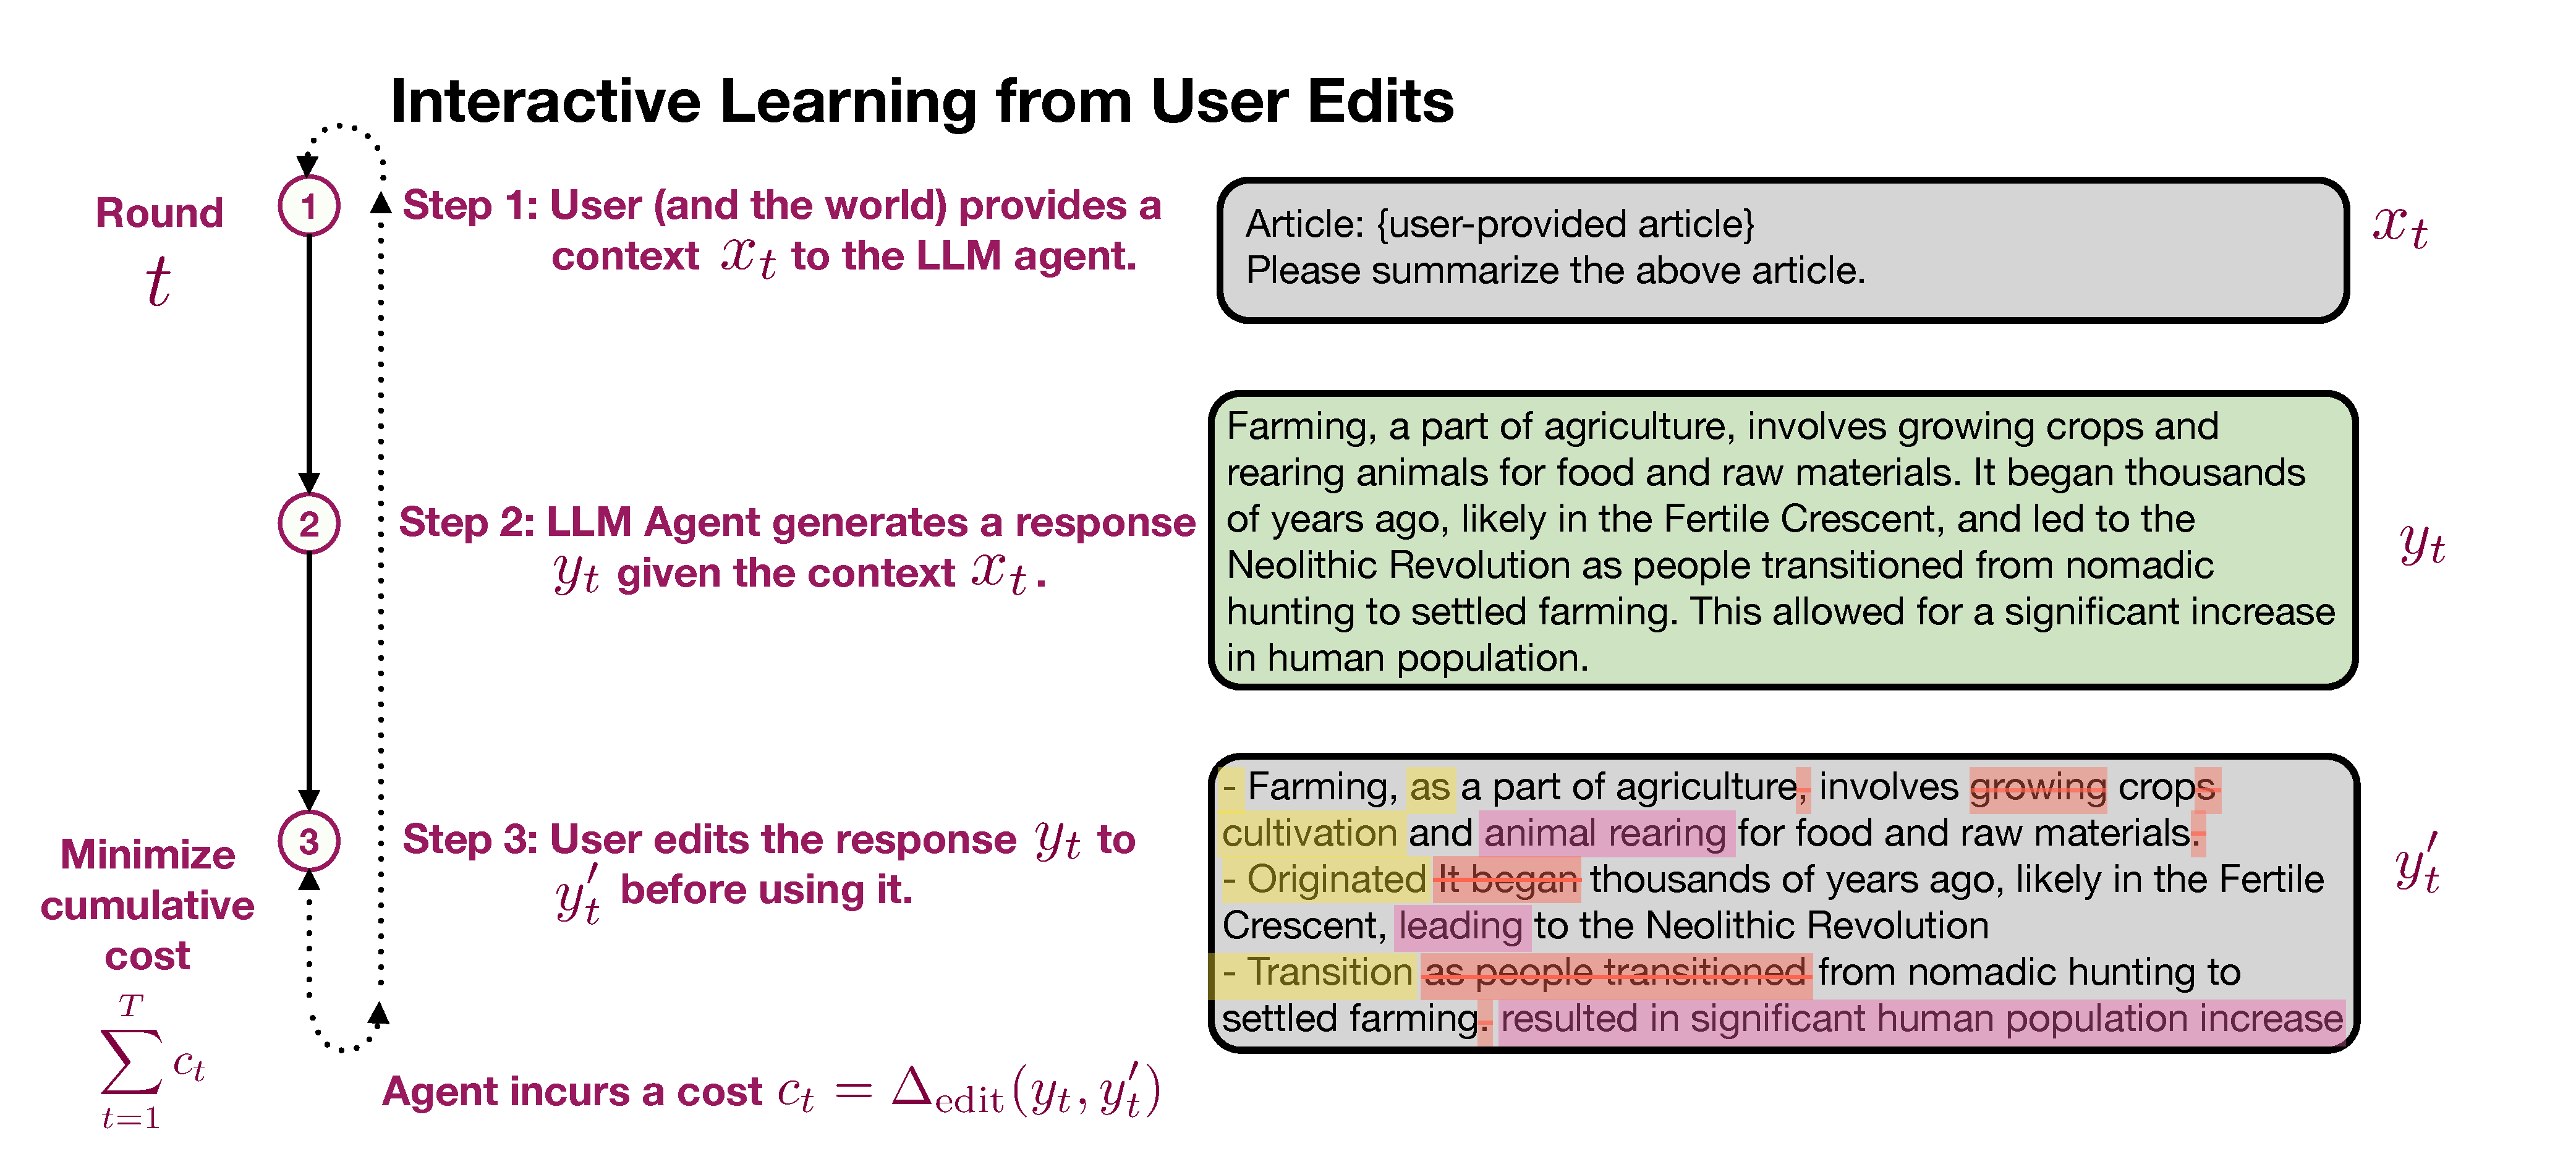
\includegraphics[clip, trim=1cm 0.5cm 3.5cm 1cm, width=1.00\textwidth]{graphs/main_diagram_vertical.pdf} 
    \caption{Illustration of interactive learning from user edits. Color coding in edits is for visualization only -- our agent takes the plain revised text as feedback. }
    \label{fig:main}
    \vspace{-15pt}
\end{figure*}

Consider the scenario in~\pref{fig:main} where a user interacts with an LLM-based writing assistant (agent) to complete their task. The interaction starts with the user (and the world) providing a context to the agent. This context may include a query prompt provided by the user, along with additional information provided by the world, such as the content on the screen, current time, and the user's calendar information. The agent generates a textual response to the user given the context.

In the beginning, the agent's response may not be optimal for the user, as it is not personalized to this user's individual needs and preference. As most users are not familiar with prompt engineering, and LLMs are often able to generate an acceptable response for the task, therefore, users may find it the most convenient to simply edit the response when it is not ideal to suit their needs, rather than trying different prompts to get new responses. The example in~\pref{fig:main} illustrates that the user directly edits the summary generated by the agent to satisfy their preference on bullet point format. It takes time and efforts for the user to make edits. We can measure such cost using a variety of metrics, such as the edit distance between the agent-generated response and the user-revised text. Zero edit from the user is also a useful feedback, reflecting that the agent's response satisfies this user's needs. One important feature of our setting is that \emph{every natural use of the agent yields an edit feedback for learning}. Since there is no distinction between training and testing in this setting, we care about minimizing the user's efforts across all rounds of interaction with the agent.
In summary, our goal is to learn from the implicit feedback in user edit history to minimize the cumulative cost of the user's efforts.\looseness=-1

We conjecture that user edits are driven by user's hidden preference which can be described in natural language. These \emph{preference descriptions} are different from the notion of comparison-based preference used in RLHF. In this paper, we use the word \emph{preference} to mean \emph{preference descriptions}. For instance, preference of the user in~\pref{fig:main} can be described as \emph{bullet points}. In practice, user preference can be compound, such as preferring \emph{bullet point, informal, with emojis} at the same time, and also context-dependent, e.g., \emph{informal} tone when writing an email to a family member, and \emph{formal} tone when writing to a colleague. In more complex settings, user preference can evolve with time (non-stationary), or depend on information unavailable in the context (partially observed). Such user preference may not be fully derivable from the context, and the user may not even be fully aware of all their preference. These considerations imply that user preference is \emph{latent} to the language agent. If the agent could learn the \emph{latent} preference correctly, it can significantly improve its performance by generating satisfactory responses accordingly. Furthermore, preference learned by the agent can be shown to the user to enhance \emph{interpretability}, and can even be modified by the user to improve correctness. Motivated by this, we propose a learning framework, \textbf{\framework} (\textbf{PRE}ference \textbf{L}earning from \textbf{U}ser's \textbf{D}irect \textbf{E}dits), where we seek to learn a textual description of the user preference for a given context using the history of user edits.

In a typical real-world scenario such as writing assistants, one has to potentially update the LLM-based agent for every user. Efficient approaches, therefore, must scale with the number of users. This makes approaches that perform a full fine-tuning of the LLM used by the agent very hard to scale. Furthermore, LLMs typically undergo evaluation on a variety of metrics before being released, and thus fine-tuning them often results in breaking the generalization guarantees offered by these tests. For example, fine-tuning GPT-4 for millions of users can quickly turn very expensive. Approaches such as adding LORA and Adapter layers and only updating them, or using federated learning, can reduce the expense to some extent, while the loss of generalizable alignment remains as a concern. In this work, we focus on leveraging a frozen, black-box LLM, and instead learning a \emph{prompt policy} that can infer textual description of user's preference for a given context, and then use it to directly drive the response generation.

We introduce a simple yet effective algorithm~\textbf{\algname}~(\textbf{C}onsolidates \textbf{I}nduced \textbf{P}references based on \textbf{H}istorical \textbf{E}dits with \textbf{R}etrieval) under the \framework~framework. For a given context,~\algname~first retrieves the $k$-closest contexts from history, and aggregates inferred preferences for these $k$ contexts. It relies on this aggregate preference to generate a response for the given context. If the user performs no edits, then it saves this aggregate preference as the correct preference for the given context. Otherwise, it queries the LLM to infer a plausible preference that explains these user edits made to the agent response, and saves this inferred preference as the correct preference for the given context. A key advantage of~\algname~is that it typically leads to significantly shorter prompts compared to other retrieval methods that use the entire documents or context, as inferred preferences are much shorter than retrieved documents or contexts. This results in a significant reduction in the computational expense of querying the LLM.

We introduce two interactive environments for evaluation, inspired by writing assistant applications. In the first environment, we evaluate the agent's ability to summarize a given document (articles from different sources). In the second environment, we evaluate the agent's ability to compose an email using content from a given document (notes for various purpose). In both tasks, we simulate a GPT-4 user that can generate edits based on a pre-designed \emph{latent} preference. We use documents from several existing domains as our user-provided context, and vary the GPT-4 user's preference based on the domain, in order to capture the real-world context-dependent nature of human user's preference. We evaluate \algname~against several baselines, including approaches that learn context-agnostic user preferences, and retrieval-based approaches that do not learn preferences but directly use past user edits for generation. We show that for both tasks, \algname~achieves the lowest user edit cost compared to baselines, and significantly reduces the cumulative cost compared to using the frozen base agent. Additionally, \algname~results in a lower LLM query cost than other retrieval-based baselines.
Finally, we qualitatively and quantitatively analyze preferences learned by our agents, and find that they show significant similarity to the ground truth latent preferences in our setup.














\section{Relative Term Rewriting}\label{Relative Term Rewriting}

We assume familiarity with term rewriting \cite{baader_nipkow_1999} and regard (finite) TRSs
over a (finite) signature $\Sigma$ and a set of variables $\VSet$.

\begin{example}\label{ex:divlTRS}
Consider the following TRS $\R_{\tdivl}$, where $\tdivl(x,\xs)$ computes the
number that results from dividing $x$ by each element of the list $\xs$. 
As usual, natural numbers are 
represented by the function symbols $\O$ and $\ts$, and lists are represented via $\tnil$
and $\tcons$. 
Then $\tdivl(\ts^{24}(\O), \tcons(\ts^4(\O), \tcons(\ts^3(\O),\tnil)))$ evaluates to
$\ts^2(\O)$, because $(24/4)/3 = 2$. Here, $\ts^2(\O)$ stands for $\ts(\ts(\O))$, etc.

\vspace*{-0.5cm}

{\footnotesize
\hspace*{-0.85cm}
\begin{minipage}[t]{5.1cm}
    \begin{align}
        \label{R-minus-rule-2} \tminus(x,\O) &\to x\\
        \label{R-minus-rule-1} \tminus(\ts(x),\ts(y)) &\to \tminus(x,y) \\
        \label{R-div-rule-1} \tdiv(x,\ts(\O)) &\to x\!
    \end{align}
\end{minipage}\hspace{.3cm}
\begin{minipage}[t]{7.1cm}
    \begin{align}
        \label{R-div-rule-2} \tdiv(\ts(x),\ts(y)) &\to \ts(\tdiv(\tminus(x,y),\ts(y)))\\
        \label{R-list-rule-2} \tdivl(x,\tnil) &\to x \\
        \label{R-list-rule-1} \tdivl(x,\tcons(y,\xs)) &\to \tdivl(\tdiv(x,y),\xs) \!
         \end{align}
\end{minipage}}
\end{example}

\smallskip

\noindent 
A TRS $\R$ induces a \emph{rewrite relation} ${\to_{\R}} \subseteq \TSet{\Sigma}{\VSet}
\times \TSet{\Sigma}{\VSet}$ on terms where $s \to_{\R} t$ holds if there is a position
 $\pi \in \pos(s)$, 
a rule $\ell \to r \in \R$, and a substitution $\sigma$ such that $s|_{\pi}=\ell\sigma$ and $t = s[r\sigma]_{\pi}$.
For example, we have $\tminus(\ts(\O),\ts(\O)) \to_{\R_{\tdivl}} \tminus(\O,\O) \to_{\R_{\tdivl}} \O$.
We call a TRS $\R$ \emph{strongly normalizing (SN)} or \emph{terminating} if $\to_{\R}$ is
well founded. Using the DP framework, one can easily prove that
$\R_{\tdivl}$ is SN (see \Cref{Dependency Pairs for Ordinary Term Rewriting}). In
particular, in each application of the recursive $\tdivl$-rule 
\eqref{R-list-rule-1}, the length of the list in $\tdivl$'s second argument is
decreased by one.

In the relative setting, one considers two TRSs
$\R$ and $\R^{=}$.
We say that $\R$ is \emph{relatively strongly normalizing} w.r.t.\ $\R^{=}$ (i.e.,
$\R / \R^{=}$ is SN) if there is no infinite $(\to_{\R} \cup \to_{\R^{=}})$-rewrite sequence that uses an infinite number of $\to_{\R}$-steps.
We refer to $\R$ as the \emph{main} and $\R^{=}$ as the \emph{base} TRS.

\begin{example}\label{ex:mset1}
    For example, let $\R_{\tdivl}$ be the \emph{main} TRS.
    Since the order of the list elements does not affect \pagebreak[2] the termination
   of $\R_{\tdivl}$, 
     this algorithm also works for multisets.
   To abstract lists to multisets, we add the \emph{base} TRS $\R^{=}_{\tset} = \{\eqref{B-com-rule-1}\}$.
    \begin{equation}
        \label{B-com-rule-1} \tcons(x, \tcons(y,\zs)) \to \tcons(y, \tcons(x,\zs)) 
    \end{equation}
    $\R^{=}_{\tset}$ is non-terminating, since it can
    switch elements in a list arbitrarily often.
    How-\linebreak ever, $\R_{\tdivl} / \R^{=}_{\tset}$ is SN as each application of
    Rule \eqref{R-list-rule-1} still reduces the list length.
\end{example}

We will use the following four examples to show why a naive
adaption of dependency pairs does not work in the relative setting and why we need our new
notion of \emph{annotated dependency pairs}.
These examples represent different types of infinite rewrite sequences
that lead to non-termination in the relative setting: \emph{redex-duplicating},
\emph{redex-creating} (or ``-emitting''), and \emph{ordinary infinite sequences}.

\begin{example}[Redex-Duplicating]\label{example:redex-duplicating}
    Consider the TRSs $\R_1 = \{\ta \to \tb\}$ and $\R_1^{=} = \{\tf(x) \to \tc(\tf(x),x)\}$.
    $\R_1 / \R_1^{=}$ is not SN due to the infinite rewrite sequence $\underline{\tf(\ta)}
    \to_{\R_1^{=}}\linebreak \tc(\tf(\ta),\underline{\ta}) \to_{\R_1} \tc(\underline{\tf(\ta)},\tb) \to_{\R_1^{=}}
    \tc(\tc(\tf(\ta),\underline{\ta}),\tb)\to_{\R_1}
      \tc(\tc(\tf(\ta),\tb),\tb)\to_{\R_1^{=}}
    \ldots$\
    The reason is that $\R_1^{=}$ can be used to duplicate an arbitrary $\R_1$-redex infinitely often.
\end{example}

\begin{example}[Redex-Creating on Parallel Position]\label{example:redex-creating}
    Next, consider $\R_2 = \{\ta \to \tb\}$ and $\R_2^{=} = \{\tf \to \tc(\tf,\ta)\}$.
    $\R_2 / \R_2^{=}$ is not SN as we have the infinite rewrite sequence $\underline{\tf}
    \to_{\R_2^{=}} \tc(\tf,\underline{\ta}) \to_{\R_2} \tc(\underline{\tf},\tb) \to_{\R_2^{=}}
    \tc(\tc(\tf,\underline{\ta}),\tb) \to_{\R_2}
 \tc(\tc(\underline{\tf},\tb),\tb) \to_{\R_2^{=}} \ldots$\
 Here, $\R_2^{=}$ can create an
 $\R_2$-redex infinitely often (where
 in the right-hand side $\tc(\tf,\ta)$ of $\R_2^{=}$'s rule, the
 $\R_2^=$-redex $\tf$ and
 the created $\R_2$-redex $\ta$ are on parallel positions).
\end{example}

\begin{example}[Redex-Creating on Position Above]\label{example:redex-creatingAbove}
  Let $\R_3 = \{\ta(x) \to \tb(x)\}$ and $\R_3^{=} = \{\tf \to \ta(\tf)\}$.
    $\R_3 / \R_3^{=}$ is not SN as we have $\underline{\tf} \to_{\R_3^{=}}
    \underline{\ta}(\tf) \to_{\R_3} \tb(\underline{\tf}) \to_{\R_3^{=}}
    \tb(\underline{\ta}(\tf)) \to_{\R_3} 
 \tb(\tb(\underline{\tf})) \to_{\R_3^{=}}\ldots$, i.e., again
    $\R_3^{=}$ can be used to create an
 $\R_3$-redex infinitely often.
 In the right-hand side $\ta(\tf)$ of
$\R_3^=$'s rule,
the position  of the created $\R_3$-redex $\ta(\ldots)$
    is above the position of the  $\R_3^=$-redex $\tf$.
\end{example}

  

\begin{example}[Ordinary Infinite]\label{example:ordinary-infinite}
  Finally, consider $\R_4 = \{\ta \to \tb\}$ and $\R_4^{=} = \{ \tb \to \ta\}$.
Here, the base TRS $\R_4^{=}$ can neither duplicate nor create an $\R_4$-redex infinitely often,
    but in combination with the main TRS $\R_4$ we obtain the
  infinite rewrite sequence $\ta \to_{\R_4}
    \tb \to_{\R_4^{=}} \ta \to_{\R_4}
    \tb \to_{\R_4^{=}} \ldots$\ Thus,
    $\R_4 / \R_4^{=}$ is not SN. 
\end{example}


\section{DP Framework}\label{DP Framework}

We first recapitulate dependency pairs for ordinary (non-relative) rewriting in \Cref{Dependency Pairs for Ordinary Term Rewriting}
and summarize existing results on DPs for relative rewriting in \Cref{Dependency Pairs for Relative Termination}.

\subsection{Dependency Pairs for Ordinary Term Rewriting}\label{Dependency Pairs for Ordinary Term Rewriting}

We recapitulate DPs and the two most important processors of the DP framework, and refer to, e.g.,
\cite{arts2000termination,gieslLPAR04dpframework,giesl2006mechanizing,hirokawa2005automating,DBLP:journals/iandc/HirokawaM07}
for more details.
As an example, we show how to prove termination of $\R_{\tdivl}$ without the base $\R^{=}_{\tset}$.
We decompose the signature
$\Sigma =  \SignatureC \uplus  \SignatureD$ of a TRS $\R$ 
such that $f \in \SignatureD$ if $f = \rootsym(\ell)$ for some rule $\ell \to r \in \R$.
The symbols in $\SignatureC$ and $\SignatureD$ are called 
\emph{constructors} and \emph{defined symbols} of $\R$, respectively. 
For every $f \in \SignatureD$, we introduce a fresh \emph{annotated symbol} $f^{\#}$ of the same arity.
Let $\SignatureA$ denote the set of all annotated symbols, and $\SignatureADC = \Sigma \uplus \SignatureA$.
To ease readability, we often use capital letters like $\tF$ instead of $\tf^\#$.
For any term $t = f(t_1,\ldots,t_n) \in \TSet{\Sigma}{\VSet}$ with $f \in \SignatureD$, 
let $t^{\#} = f^{\#}(t_1,\ldots,t_n)$.
For a rule $\ell \to r$ and each subterm $t$ of $r$ with \pagebreak[2] defined root symbol, one obtains a
\emph{dependency pair} $\ell^\# \to t^\#$.
Let $\DPair{\R}$ denote the set of all dependency pairs of the TRS $\R$.

\begin{example}
  \label{example:dependency-pair}
    For $\R_{\tdivl}$ from \Cref{ex:divlTRS}, we obtain the following five dependency pairs.

    \vspace*{-.5cm}
    
    {\footnotesize
    \hspace*{-.9cm}
    \begin{minipage}[t]{5.7cm}
             \begin{align}
          \label{R-div-deppair-3} \tM(\ts(x),\ts(y)) &\to \tM(x,y) \\
            \label{R-div-deppair-2} \tD(\ts(x),\ts(y)) &\to \tM(x,y) \\
           \label{R-div-deppair-1} \tD(\ts(x),\ts(y)) &\to \tD(\tm(x,y),\ts(y))        
            \end{align}
    \end{minipage}\hspace*{.3cm}
    \begin{minipage}[t]{6.6cm}
        \begin{align}
            \label{R-div-deppair-4} \tDL(x,\tcons(y,\xs)) &\to \tD(x,y) \\
            \label{R-div-deppair-5} \tDL(x,\tcons(y,\xs)) &\to \tDL(\tdiv(x,y),\xs) 
        \end{align}
    \end{minipage}}
\end{example}

The DP framework operates on \emph{DP problems} $(\C{P}, \R)$ where
$\C{P}$ is a (finite) set of DPs, and $\R$ is a (finite) TRS. 
A (possibly infinite) sequence $t_0, t_1, t_2,
\ldots$ with $t_i \rootto_{\C{P}} \circ \to_{\R}^* t_{i+1}$ for all $i$ is a $(\C{P}, \R)$-\emph{chain}.
Here, $\rootto$ denotes rewrite steps at the root.
Intuitively, a chain represents subsequent ``function calls''  in evaluations. 
Between two function calls (corres\-ponding to steps with $\C{P}$, called $\mathbf{p}$-steps) one can evaluate the
arguments using arbitrary many steps with $\R$ (called $\mathbf{r}$-steps).
So $\mathbf{r}$-steps are rewrite steps that are needed in order to enable another
$\mathbf{p}$-step at a position above later on.\linebreak
For example, $\tDL(\ts(\O), \tcons(\ts(\O), \tnil)), \tDL(\ts(\O),\tnil)$ is a
$(\DPair{\R_{\tdivl}}, \R_{\tdivl})$-chain, as $\tDL(\ts(\O), \tcons(\ts(\O), \tnil))
\rootto_{\DPair{\R_{\tdivl}}} \tDL(\tdiv(\ts(\O),\ts(\O)),\tnil) \to_{\R_{\tdivl}}^*\!\tDL(\ts(\O),\tnil)$.

A DP problem $(\C{P}, \R)$ is called
\emph{strongly normalizing (SN)} if there is no infinite $(\C{P}, \R)$-chain.
The main result on DPs is the \emph{chain criterion} which states that a TRS
$\R$ is SN iff $(\DPair{\R}, \R)$ is SN.
The key idea of the DP framework is a \emph{divide-and-conquer} approach which
applies \emph{DP processors} to transform DP problems into simpler sub-problems.
A \emph{DP processor} $\Proc$ has the form $\Proc(\C{P}, \R) = \{(\C{P}_1,\R_1), \ldots, (\C{P}_n,\R_n)\}$, 
where $\C{P}, \C{P}_1, \ldots, \C{P}_n$ are sets of DPs and $\R, \R_1, \ldots, \R_n$ are TRSs. 
$\Proc$ is \emph{sound} if $(\C{P}, \R)$ is SN whenever 
$(\C{P}_i,\R_i)$ is SN for all $1 \leq i \leq n$. 
It is \emph{complete} if $(\C{P}_i,\R_i)$ is SN for all 
$1 \leq i \leq n$ whenever $(\C{P}, \R)$ is SN.


So for a TRS $\R$, one starts with the initial
DP problem $(\DPair{\R}, \R)$ and applies sound 
(and preferably complete) DP processors until all sub-problems are ``solved'' (i.e.,
DP processors transform them to the empty set).
This allows for modular ter-\linebreak mination
proofs, as different techniques can be applied on each sub-problem $(\C{P}_i, \R_i)$.

One of the most important processors is the \emph{dependency graph processor}.
The \emph{$(\C{P}, \R)$-dependency graph} indicates
which DPs can be used after each other in  
chains.\linebreak
Its nodes are $\C{P}$ and there is an edge from $s_1 \to t_1$ to $s_2 \to t_2$ if there
are substitutions
\begin{wrapfigure}[5]{r}{0.14\textwidth}
  \begin{center}
  \scriptsize
    \vspace*{-1.3cm}
    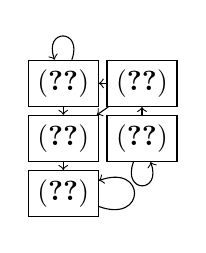
\begin{tikzpicture}
        \node[shape=rectangle,draw=black!100] (A) at (1,0.7) {\eqref{R-div-deppair-5}};
        \node[shape=rectangle,draw=black!100] (B) at (1,1.4) {\eqref{R-div-deppair-4}};
        \node[shape=rectangle,draw=black!100] (C) at (0,0) {\eqref{R-div-deppair-3}};
        \node[shape=rectangle,draw=black!100] (D) at (0,.7) {\eqref{R-div-deppair-2}};
        \node[shape=rectangle,draw=black!100] (E) at (0,1.4) {\eqref{R-div-deppair-1}};
   
        \path [->,in=290,out=250,looseness=5] (A) edge (A);
        \path [->] (A) edge (B);
        \path [->] (B) edge (D);
        \path [->] (B) edge (E);
        \path [->,in=20,out=340,looseness=5] (C) edge (C);
        \path [->] (D) edge (C);
        \path [->] (E) edge (D);
        \path [->,in=110,out=70,looseness=5] (E) edge (E);
    \end{tikzpicture}
    \caption*{}
  \end{center}
\end{wrapfigure}
$\sigma_1, \sigma_2$ with $t_1 \sigma_1 \to_{\R}^* s_2 \sigma_2$.
The $(\DPair{\R_{\tdivl}}, \R_{\tdivl})$-dependency graph is on the right.
Any infinite $(\C{P}, \R)$-chain corresponds to
an infinite path in the dependency graph, and since the graph is finite, this infinite
path must end in a strongly connected component (SCC).\footnote{Here, a
set $\C{P}'$ of dependency pairs is  an \emph{SCC} if it is a maximal cycle,
i.e., it is a maximal set such that for any $s_1 \to t_1$ and $s_2 \to
t_2$ in $\C{P}'$ there is
a non-empty path from $s_1 \to t_1$ to $s_2 \to
t_2$ which only traverses nodes from $\C{P}'$.}
Hence, it suffices to consider the SCCs of this graph independently.

\begin{restatable}[Dep.\ Graph Processor]{theorem}{depgraph}\label{DGP}
    For the SCCs $\C{P}_1, \ldots, \C{P}_n$ of the $(\C{P}, \R)$-dependency graph,  
    $\Proc_{\mathtt{DG}}(\C{P},\R) = \{(\C{P}_1,\R), \ldots, (\C{P}_n,\R)\}$ is sound and complete. 
\end{restatable}

While the exact dependency graph is not computable in general, there are 
techniques to over-approximate it automatically, see, e.g.,
\cite{arts2000termination,giesl2006mechanizing,hirokawa2005automating}.
In our example, $\Proc_{\mathtt{DG}}(\DPair{\R_{\tdivl}}, \R_{\tdivl})$ yields
$\bigl(\{\eqref{R-div-deppair-3}\}, \R_{\tdivl}\bigr)$,
$\bigl(\{\eqref{R-div-deppair-1}\}, \R_{\tdivl}\bigr)$,
 and $\bigl(\{\eqref{R-div-deppair-5}\}, \R_{\tdivl}\bigr)$.

The second crucial processor adapts classical reduction orders to DP problems.
A \emph{reduction pair} $(\succsim, \succ)$ consists of two \pagebreak[2]
relations on terms such that $\succsim$
is reflexive, transitive, and
closed under contexts and substitutions, and $\succ$ is a well-founded
order that is closed under substitutions but does
not have to be closed under contexts.
Moreover, $\succsim$ and $\succ$ must be compatible, 
i.e., ${\succsim} \circ {\succ} \circ {\succsim} \, \subseteq \, {\succ}$.
The \emph{reduction pair processor}
requires that all rules and dependency pairs are weakly decreasing,
and it removes those DPs that are strictly decreasing.

\begin{restatable}[Reduction Pair Processor]{theorem}{rpp}\label{RPP}
    Let $(\succsim, \succ)$ be a reduction pair such that $\C{P} \cup \R \subseteq \, \succsim$.
    Then $\Proc_{\mathtt{RPP}}(\C{P},\R) = \{(\C{P} \, \setminus \succ, \R)\}$ is sound and complete.
\end{restatable}

For example, one can use reduction pairs based on
polynomial interpretations \cite{lankford1979proving}.
A \emph{polynomial interpretation} $\Pol$ is a $\SignatureADC$-algebra which maps every
function symbol $f \in \SignatureADC$ to a polynomial $f_{\Pol} \in \IN[\VSet]$.
$\Pol(t)$ denotes the \emph{interpretation} of a term $t$ by the $\SignatureADC$-algebra $\Pol$.
Then $\Pol$ induces a reduction pair
$(\succsim, \succ)$ where $t_1 \succsim t_2$ ($t_1 \succ t_2$) holds if the inequation $\Pol(t_1) \geq \Pol(t_2)$
($\Pol(t_1) > \Pol(t_2)$) is true for all
instantiations of its variables by natural numbers.



For the three remaining
DP problems in our example, we can apply
the reduction pair processor using
the polynomial interpretation
which maps $\O$ to $0$, $\ts(x)$ to $x + 1$,
$\tcons(y,\xs)$ to $\xs + 1$, $\tDL(x,\xs)$ to $\xs$,
and all other symbols to their first arguments. 
Since $\eqref{R-div-deppair-3}$, $\eqref{R-div-deppair-1}$,
and $\eqref{R-div-deppair-5}$ are strictly decreasing, 
$\Proc_{\mathtt{RPP}}$ transforms all three remaining DP problems 
into DP problems of the form $(\emptyset, \ldots)$. 
As $\Proc_{\mathtt{DG}}(\emptyset, \ldots) = \emptyset$ 
and all processors used are sound, this means that there is no
infinite chain for the initial DP problem 
$(\DPair{\R_{\tdivl}}, \R_{\tdivl})$ and thus, $\R_{\tdivl}$ is SN.

\subsection{Dependency Pairs for Relative Termination}\label{Dependency Pairs for Relative Termination}

Up to now, we only considered DPs for ordinary termination of TRSs.
The easiest idea to use DPs in the relative setting is to start with the DP problem 
$(\DPair{\R \cup \R^{=}}, \R \cup \R^{=})$.
This would prove termination of $\R \cup \R^{=}$, which implies termination of $\R / \R^{=}$, but
ignores that the rules in $\R^{=}$ do not have to terminate.
Since termination of DP problems is already defined via a relative condition (finite chains
can only have finitely
many $\mathbf{p}$-steps but may have
infinitely many $\mathbf{r}$-steps),
another idea 
for proving termination of $\R / \R^{=}$ is to start
with the DP problem $(\DPair{\R}, \R \cup \R^{=})$, which only considers
the DPs of $\R$.
However,  this is unsound in general.

\begin{example}\label{ex:dps-dont-work-in-relative}
     The only defined symbol of $\R_2$  from \Cref{example:redex-creating} is $\ta$.
     Since the right-hand side of $\R_2$'s rule does not contain 
  defined symbols, we would get the DP problem
  $(\emptyset,\linebreak \R_2 \cup \R_2^{=})$, which is SN as it has no
  DP.
    Thus, we would falsely conclude that $\R_2 / \R_2^{=}$\linebreak is SN.
Similarly, 
this approach would also falsely ``prove'' SN for
\Cref{example:redex-duplicating,example:redex-creatingAbove}.
\end{example}

In \cite{iborra2017relative}, it was shown that under
certain conditions on $\R$ and $\R^{=}$, starting with the DP problem $(\DPair{\R \cup \R_a^{=}},
\R \cup \R^{=})$ for a subset $\R_a^{=} \subseteq \R^{=}$
is sound
for relative termination.\footnote{As before,
for the construction of $\DPair{\R
  \cup \R_a^{=}}$,  only the root symbols of left-hand sides of $\R
\cup \R_a^{=}$
are considered to be ``defined''.}
The two restrictions on the TRSs are \emph{dominance} and being \emph{non-duplicating}.
We say that $\R$ \emph{dominates} $\R^{=}$ if defined symbols of $\R$
do not occur in
the right-hand sides of rules of $\R^{=}$.
A TRS is \emph{non-duplicating} if no variable occurs more often
on the right-hand side of a rule than on its left-hand side.

\begin{restatable}[First Main Result of~\cite{iborra2017relative}, Sound and Complete]{theorem}{main-relative-rewrite-corollary-yamada-1}\label{theorem:main-relative-rewrite-corollary-yamada-1}
    Let $\R$ and $\R^{=}$ be TRSs such that $\R^{=}$ is non-duplicating and \pagebreak[2] $\R$ dominates $\R^{=}$.
    Then the DP problem
      $(\DPair{\R}, \R \cup \R^{=})$ is SN iff $\R / \R^{=}$ is SN.
\end{restatable}

\begin{restatable}[Second Main Result of~\cite{iborra2017relative}, only Sound]{theorem}{main-relative-rewrite-corollary-yamada-2}\label{theorem:main-relative-rewrite-corollary-yamada-2}
    Let $\R$ and $\R^{=} = \R^{=}_a \uplus \R^{=}_b$ be TRSs.
	If $\R^{=}_b$ is non-duplicating, $\R \cup \R^{=}_a$ dominates $\R^{=}_b$,
    and the DP problem $(\DPair{\R \cup \R^{=}_a}, \R \cup \R^{=})$ is SN, 
    then $\R / \R^{=}$ is SN.
\end{restatable}

\begin{example}
  For the main TRS $\R_{\tdivl}$ from \Cref{ex:divlTRS} and base TRS $\R^{=}_{\tset}$ from \Cref{ex:mset1}\linebreak
  we can apply
    \Cref{theorem:main-relative-rewrite-corollary-yamada-1} and consider the DP problem
    $(\DPair{\R_{\tdivl}}, \R_{\tdivl} \cup \R^{=}_{\tset})$, since $\R^{=}_{\tset}$ is
    non-duplicating and $\R_{\tdivl}$ dominates $\R^{=}_{\tset}$.
    As for $(\DPair{\R_{\tdivl}}, \R_{\tdivl})$, the DP
    framework can prove that $(\DPair{\R_{\tdivl}}, \R_{\tdivl} \cup
    \R^{=}_{\tset})$ is SN. In this way, the tool \natt{} 
    which implements the results of
    \cite{iborra2017relative}  proves that $\R_{\tdivl} / \R^{=}_{\tset}$ is SN.
In contrast,  a direct application of  simplification orders fails to prove
    SN for $\R_{\tdivl} / \R^{=}_{\tset}$ because simplification orders already fail to
    prove termination of $\R_{\tdivl}$.
\end{example}

\begin{example}\label{ex:mainExample}
    If we consider $\R^{=}_{\tset 2}$ with the rule 
    \begin{equation}
        \label{B-com-rule-2} \tdivl(z,\tcons(x, \tcons(y,\zs))) \to \tdivl(z,\tcons(y, \tcons(x,\zs)))
    \end{equation}
    instead of $\R^{=}_{\tset}$ as the base TRS, then $\R_{\tdivl} / \R^{=}_{\tset 2}$ remains strongly normalizing,
    but we cannot use \Cref{theorem:main-relative-rewrite-corollary-yamada-1} since $\R_{\tdivl}$ does not
    dominate $\R^{=}_{\tset 2}$. If we try to split $\R^{=}_{\tset 2}$ as in
    \Cref{theorem:main-relative-rewrite-corollary-yamada-2}, then
    $\emptyset \neq \R^{=}_a \subseteq \R^{=}_{\tset 2}$ implies $\R^{=}_a = \R^{=}_{\tset
    2}$, but
    $\R^{=}_{\tset  2}$ is 
    non-terminating.
    Therefore, all previous tools for relative termination fail in proving that $\R_{\tdivl} /
    \R^{=}_{\tset 2}$ is SN.
    In \Cref{Relative DP Framework} we will present our novel DP framework which can prove
    relative termination of relative TRSs 
    like $\R_{\tdivl} / \R^{=}_{\tset 2}$.
\end{example}

As remarked in \cite{iborra2017relative},
\Cref{theorem:main-relative-rewrite-corollary-yamada-1,theorem:main-relative-rewrite-corollary-yamada-2} 
are unsound if one only considers \emph{minimal} chains, i.e., if
for a DP problem $(\C{P},\R)$ one only considers 
chains $t_0, t_1, \ldots$, where all\linebreak $t_i$ are $\R$-strongly normalizing.
In the DP framework for ordinary rewriting,
the re\-striction to minimal chains allows the use of further processors, e.g., based on
\emph{usable}\linebreak \emph{rules} \cite{giesl2006mechanizing,DBLP:journals/iandc/HirokawaM07} or the \emph{subterm criterion} \cite{DBLP:journals/iandc/HirokawaM07}.
As shown in \cite{iborra2017relative}, usable rules and the subterm
criterion can nevertheless be 
applied if $\R^{=}$ is \emph{quasi-terminating} \cite{dershowitz_termination_1987}, 
i.e., the\linebreak set $\{t \mid s \to_{\R^{=}}^* t \}$ is finite for every term $s$.
This restriction would also be needed to integrate processors that rely on
minimality
into our new framework in \Cref{Relative DP Framework}.

\section{Annotated Dependency Pairs for Relative Termination}\label{Relative DP Framework}



As shown in \Cref{Dependency Pairs for Relative Termination},
up to now there only exist criteria \cite{iborra2017relative} that state
when it is sound to apply
\emph{ordinary} DPs for proving relative termination, but there is no \emph{specific} DP-based technique
to analyze relative termination directly. To solve this problem, we now
adapt the concept of \emph{annotated dependency pairs} (ADPs) for relative termination.
ADPs were introduced in \cite{FLOPS2024} to prove innermost almost-sure termination of probabilistic term rewriting.
In the relative setting, we can use similar dependency pairs as in the probabilistic setting,
but with a different rewrite relation $\tored{}{}{}$ to deal with non-innermost rewrite steps.
Compared to \cite{iborra2017relative},
we can (a) remove the requirement of dominance, which will be handled
by the dependency graph processor, and (b) allow for ADP processors that are specifically designed for the relative
setting before possibly moving to ordinary DPs.
The requirement that 
$\R^{=}$ must be non-duplicating remains, since DPs do not help in analyzing
redex-duplicating sequences as in \Cref{example:redex-duplicating}, where the crucial redex
$\ta$ is not generated from a ``function call'' \pagebreak[2]
in the right-hand side of a rule,
but it just corresponds to a duplicated variable.
To handle TRSs $\R / \R^{=}$ where $\R^{=}_{dup} \subseteq\R^{=}$
is duplicating,
one can move the duplicating rules to the main TRS $\R$ and 
try to prove relative termination of
$(\R \cup \R^{=}_{dup})/(\R^{=} \setminus \R^{=}_{dup})$ instead,
or one can try to find a reduction pair $(\succsim, \succ)$ where
$\succ$ is closed under contexts such that $\R \cup \R^= \subseteq {\succsim}$ and
$\R^{=}_{dup} \subseteq {\succ}$. Then it suffices to prove relative termination of $(\R
\setminus \succ, \R^{=} \setminus \succ)$ instead.



For ordinary termination, we create a separate DP for each occurrence of a
defined symbol in the right-hand side of a rule (and no DP is created for rules without
defined symbols in their right-hand sides).
This would work to detect
\emph{ordinary infinite} sequences
like the one in \Cref{example:ordinary-infinite}
in the relative setting, i.e., such an infinite sequence would give rise to an infinite chain. 
However,  as shown in \Cref{ex:dps-dont-work-in-relative}, this
would not suffice to detect infinite redex-creating sequences as in
\Cref{example:redex-creating}
with   $\R_2 = \{\ta \to \tb\}$ and $\R_2^{=} = \{\tf \to \tc(\tf,\ta)\}$:
$\underline{\tf}
    \to_{\R_2^{=}} \tc(\tf,\underline{\ta}) \to_{\R_2} \tc(\underline{\tf},\tb) \to_{\R_2^{=}}
    \tc(\tc(\tf,\underline{\ta}),\tb) \to_{\R_2}
     \ldots$\

  

    
Here, (1) we need a DP for
the rule $\ta \to \tb$ to detect the reduction of the created
$\R_2$-redex $\ta$, although $\tb$ is a constructor.
Moreover,
(2) both defined symbols $\tf$ and $\ta$ in the right-hand side of
$\tf \to \tc(\tf, \ta)$ have to be considered simultaneously:
We need $\tf$ to create an infinite number of $\R_2$-redexes, and we need $\ta$ since it
is the created $\R_2$-redex.
Hence, for rules from the base TRS $\R_2^=$, we have to consider all possible pairs of
defined symbols in their right-hand sides simultaneously.\footnote{For relative
termination, it suffices to
consider \emph{pairs} of defined symbols.
The reason is that to ``track'' a non-terminating reduction, one only has
to
consider a single redex plus possibly another redex of the base
TRS which may later create a redex again.
}
This is not needed for the main TRS $\R_2$, i.e., if the $\tf$-rule were in the
main TRS, then the $\tf$ in the right-hand side could be considered separately from the $\ta$ that it generates.
Therefore, we distinguish between \emph{main} and \emph{base ADPs} (that are
generated from the main and the base TRS, respectively).



As in \cite{FLOPS2024},  we now annotate defined
symbols directly in the original rewrite rule instead of extracting annotated subterms
from its right-hand side. In this way, we may have terms containing several annotated
symbols, which 
allows us to consider pairs of defined symbols in right-hand sides
simultaneously.

\begin{definition}[Annotations]
    For $t \in \TSet{\SignatureADC}{\VSet}$ 
    and $\Sigma' \subseteq \SignatureADC \cup \VSet$, let $\pos_{\Sigma'}(t)$ be the
    set of all positions of $t$
    with symbols or variables from $\Sigma'$.
    For $\Phi \subseteq \posDT(t)$,
    $\anno_\Phi(t)$ is the variant of $t$ where the symbols at positions from $\Phi$
    are annotated and all\linebreak other annotations are removed.
    Thus, $\posT(\anno_\Phi(t)) = \Phi$, and
    $\anno_\emptyset(t)$ removes all an-\linebreak
    notations from $t$, where we often write
    $\flat(t)$ instead of $\anno_\emptyset(t)$.
    Moreover, for a singleton $\{\pi \}$, we often write $\anno_\pi$ instead of $\anno_{\{\pi\}}$.
   We write $t \trianglelefteq_{\#}^\pi s$ if
there is a $\pi \in \posT(s)$ and $t = \flat(s|_\pi)$
(i.e., $t$ results from  a subterm of $s$ with annotated root
symbol by removing its annotations). We also write $\trianglelefteq_{\#}$ instead of $\trianglelefteq_{\#}^\pi$.
\end{definition}

\begin{example}
    If $\tf \in \SignatureD$, then we have $\anno_{1}(\tf(\tf(x))) =
    \anno_{1}(\tF(\tF(x))) = \tf(\tF(x))$ and $\flat(\tF(\tF(x))) = \tf(\tf(x))$. 
    Moreover, we have $\tf(x) \trianglelefteq_{\#}^{1} \tf(\tF(x))$.
\end{example}


While in \cite{FLOPS2024} all defined symbols on the right-hand sides of rules were
annotated, 
we now define our novel variant of \emph{annotated dependency pairs}
for relative rewriting.

\begin{definition}[Annotated Dependency Pair]\label{def:Canonical-ADPs}
\hspace*{-.2cm}    A rule $\ell\!\to\!r$ with $\ell\!\in\!\TSet{\Sigma}{\VSet} \setminus\linebreak
    \VSet$, $r \in \TSet{\SignatureADC}{\VSet}$, and $\VSet(r) \subseteq \VSet(\ell)$ is
    called an
    \defemph{annotated dependency pair (ADP)}.
 
    Let $\SignatureD$ be the defined symbols of $\R \cup \R^=$, and for $n \in
    \NN$, let $\ADPair{n}{\ell \to r}  =  
    \{\ell \to\linebreak \anno_{\Phi}(r) \mid \Phi \subseteq \pos_{\SignatureD}(r), |\Phi| \leq n\}$.
\pagebreak[2]  The  \defemph{canonical main ADPs} for $\R$ are $\ADPairMain{\R} = \bigcup\limits_{\ell \to r \in \R}
  \!\!\!\!  \ADPairMain{\ell\!\to\!r}$ and  the \defemph{canonical base ADPs} for $\R^=\!$
are  $\ADPairBase{\R^{=}}\!= \!\!\!
    \bigcup\limits_{\ell \to r \in \R^=} \!\!\!\! \ADPairBase{\ell\!\to\!r}$.
\end{definition}

So the left-hand side of an ADP is just the left-hand side of the original rule.
The right-hand side  results from the right-hand side of the original rule
by replacing certain defined symbols $f$ with $f^{\#}$.
Whenever
we have two ADPs  $\ell \to \anno_{\Phi'}(r)$,
$\ell \to \anno_{\Phi}(r)$
with  $\Phi' \subset \Phi$, then
we only consider $\ell \to \anno_{\Phi}(r)$ and remove
 $\ell \to \anno_{\Phi'}(r)$.

\begin{example}\label{ADP-Divl}
    The canonical ADPs
    of \Cref{example:redex-creating} are $\ADPairMain{\R_2} = \{ \ta
    \to \tb\}$
    and $\ADPairBase{\R_2^{=}} = \{\tf \to
    \tc(\tF,\tA)\}$ and for
    \Cref{example:redex-creatingAbove} we get $\ADPairMain{\R_3} = \{ \ta(x)
    \to \tb(x)\}$
    and $\ADPairBase{\R_3^{=}} = \{\tf \to
    \tA(\tF)\}$.
    For $\R_{\tdivl}/\R^{=}_{\tset 2}$ from \Cref{ex:divlTRS,ex:mainExample},
    the ADPs $\ADPairMain{\R_{\tdivl}}$ are

\vspace*{-.4cm}
    
    {\footnotesize
    \hspace*{-.7cm}\begin{minipage}[t]{5.1cm}
        \begin{align}
            \label{R-div-adp-2} \tminus(x,\O) &\to x\\
            \label{R-div-adp-1} \tminus(\ts(x),\ts(y)) &\to \tM(x,y) \\
            \label{R-div-adp-3} \tdiv(x,\ts(\O)) &\to x\\
            \label{R-div-adp-4} \tdivl(x,\tnil) &\to x \!
        \end{align}
    \end{minipage}
    \begin{minipage}[t]{7.5cm}
        \begin{align}
            \label{R-div-adp-5} \tdiv(\ts(x),\ts(y)) &\to \ts(\tD(\tminus(x,y),\ts(y)))\\
            \label{R-div-adp-6} \tdiv(\ts(x),\ts(y)) &\to \ts(\tdiv(\tM(x,y),\ts(y)))\\
            \label{R-div-adp-7} \tdivl(x,\tcons(y,\xs)) &\to \tDL(\tdiv(x,y),\xs) \\
            \label{R-div-adp-8} \tdivl(x,\tcons(y,\xs)) &\to \tdivl(\tD(x,y),\xs) \!
        \end{align}
    \end{minipage}}
    
    \vspace*{-.1cm}
   
  
    \begin{align}
      \label{B-com-adp-2}
      \hspace*{-.2cm}
         \text{and $\ADPairBase{\R^{=}_{\tset 2}}$ contains 
      {\small $\tdivl(z, \tcons(x, \tcons(y,\zs))) \to \tDL(z, \tcons(y, \tcons(x,\zs)))$}}
    \end{align}
\end{example}


In \cite{FLOPS2024},
ADPs were only used for innermost rewriting.
We now modify their rewrite relation and define what happens 
with annotations inside the substitutions during a rewrite step.
To simulate redex-creating sequences as in \Cref{example:redex-creatingAbove}
with ADPs (where the position of the created redex $\ta(\ldots)$
is above the position of the creating redex $\tf$),
ADPs should be able to rewrite above annotated arguments
without removing their annotation (we will demonstrate that in
\Cref{ex:ADPs-for-redex-creation-2}).
Thus, for an ADP $\ell \to\linebreak r$ with $\ell|_\pi = x$, we use a 
\emph{variable reposition function (VRF)} to indicate which occur-\linebreak rence of $x$ in $r$ should
keep the annotations if one rewrites an instance of $\ell$ where the subterm at position
$\pi$ is annotated.
So a VRF maps  positions of variables in the left-hand side of a rule to
positions of the same variable in the right-hand side.

\begin{definition}[Variable Reposition Function]\label{def:Var-Repos-Func}
    Let $\ell \to r$ be an ADP.
	A function $\varphi: \pos_{\VSet}(\ell) \to \pos_{\VSet}(r) \cup \{\bot\}$ is called a
    \defemph{variable reposition function (VRF)} for
    $\ell \to r$
    iff
    $\ell|_\pi = r|_{\varphi(\pi)}$ whenever
 $\varphi(\pi) \neq \bot$.
\end{definition}

\begin{example}\label{example:rel-var-repos-function}
    For the ADP $\ta(x) \to \tb(x)$ for $\R_3$ from \Cref{example:redex-creatingAbove},
    if $x$ on position 1 of the left-hand side is instantiated by $\tF$,
    then the VRF $\varphi(1) = 1$ 
    indicates that
    this ADP rewrites $\tA(\tF)$ to $\tb(\tF)$, whereas
    $\varphi(1) = \bot$  means that
    it rewrites $\tA(\tF)$ to $\tb(\tf)$.
\end{example}

With VRFs we can define the rewrite relation for ADPs w.r.t.\ full rewriting.

\begin{definition}[$\tored{}{}{\C{P}}$]\label{def:ADP-Rewriting}
    Let $\C{P}$ be a set of ADPs.
    A term $s \in \TSet{\SignatureADC}{\VSet}$ rewrites to $t$ using $\C{P}$
    (denoted $s \tored{}{}{\C{P}} t$)
if there is a rule $\ell \to r \in \C{P}$, 
    a substitution $\sigma$, a position $\pi \in \posDT(s)$
    such that $\flat(s|_\pi) = \ell\sigma$, a VRF $\varphi$ for $\ell \to r$,
    and\footnote{\label{ADPComparison2}In \cite{FLOPS2024} there
    were two additional cases in the definition of the corresponding rewrite relation. One of
    them was needed for processors that restrict the set of rules applicable for
    $\mathbf{r}$-steps (e.g., based on usable rules), and the other case 
    was needed to
    ensure that the innermost
    evaluation strategy is not affected by the application of ADP processors. This is
    unnecessary here since we consider full rewriting. On the other hand,
     VRFs are new compared to
\cite{FLOPS2024}, since they are not needed for innermost rewriting.}
    \begin{equation*}
        \begin{array}{rll@{\quad}ll@{\qquad}l}
        t &=                  &s[\anno_{\Phi}(r\sigma)]_{\pi}  & 
        \text{if} & \pi \in \posT(s)    & (\mathbf{pr})\\ 
        t &=                  &s[\anno_{\Psi}(r\sigma)]_{\pi}  & 
        \text{if} & \pi \in\pos_\SignatureD(s) & (\mathbf{r})\!
        \end{array}
    \end{equation*}
    Here, $\Psi \!=\! \{\varphi(\rho).\tau \mid \rho \!\in\! \pos_{\VSet}(\ell), \,
    \varphi(\rho) \neq \bot,  \, \rho.\tau \!\in\! \posT(s|_{\pi}) \}$
    and $\Phi = \posT(r) \cup \Psi$.
\end{definition}
So $\Psi$ considers all positions of annotated symbols in $s|_{\pi}$ that
are below
positions $\rho$ of\linebreak variables in $\ell$. If the VRF maps $\rho$ to a variable position
$\rho'$ in
$r$, then the annotations below $\pi.\rho$ in $s$ are kept in the resulting subterm at
position $\pi.\rho'$
after the rewriting.

Rewriting with $\C{P}$ is like ordinary term rewriting, while considering and
modifying
annotations.
Note that we represent all DPs resulting from a rule as well as the original
rule by just one ADP.  
So the ADP $\tdiv(\ts(x),\ts(y)) \to \ts(\tD(\tminus(x,y),\ts(y)))$
represents both the DP resulting from $\tdiv$ in the right-hand side
of the rule \eqref{R-div-rule-2}, and the rule \eqref{R-div-rule-2} itself 
(by simply disregarding all annotations of the ADP).

Similar to the classical DP framework, our goal is to track specific reduction
sequences. As before, 
there are $\mathbf{p}$-steps where
a DP is applied at the
position of an annotated symbol. These steps may
introduce new annotations. Moreover, 
between two $\mathbf{p}$-steps there can be
several $\mathbf{r}$-steps.

A step of the form $(\mathbf{pr})$ at position $\pi$ in \Cref{def:ADP-Rewriting} 
represents  
a $\mathbf{p}$- or an  
$\mathbf{r}$-step\linebreak (or both), where an  
$\mathbf{r}$-step is only possible 
if one later rewrites an annotated symbol at a position above $\pi$.
All annotations are kept during this step except for annotations of subterms
that correspond to variables of the applied rule. Here, the used VRF $\varphi$ determines which of
these annotations are kept and which are removed.
As an example,
with the canonical ADP $\ta(x) \to \tb(x)$  from
$\ADPairMain{\R_3}$ we can rewrite
$\tA(\tF) \tored{}{}{\ADPairMain{\R_3}}  \tb(\tF)$ as in \Cref{example:rel-var-repos-function}.
Here, we have $\pi =
\varepsilon$, $\flat(s|_\varepsilon) = \ta(\tf) = \ell \sigma$, $r =
\tb(x)$, and the VRF $\varphi$ with 
$\varphi(1) = 1$ such that the annotation of $\tF$ in $\tA$'s argument is
kept in the  argument of $\tb$.

A step of the form $(\mathbf{r})$
rewrites at the position of a non-annotated defined symbol,
and represents just an $\mathbf{r}$-step.  
Hence, we remove all annotations
from the right-hand side $r$ of the ADP.
However, we may have to keep the annotations inside the substitution,
hence we move them according to the VRF.
For example, we obtain the rewrite step
$\ts(\tD(\underline{\tminus(\ts(\O),\ts(\O))},\ts(\O))) \tored{}{}{\ADPairMain{\R_\tdivl}}\ts(\tD(\tminus(\O,\O),\ts(\O)))$
using the ADP $\tminus(\ts(x),\ts(y)) 
\to \tM(x,y) \;$ \eqref{R-div-adp-1}
and any VRF.

A \emph{(relative) ADP problem} has the form
$(\C{P},\C{P}^{=})$, where $\C{P}$ and $\C{P}^{=}$ are finite sets of ADPs and $\C{P}^{=}$
is non-duplicating. 
$\C{P}$ is the set of all main ADPs and $\C{P}^{=}$ is the set of all base ADPs.
Now we can define chains in the relative setting.

\begin{definition}[Chains and Terminating ADP Problems]\label{def:relative-rewrite-chain}
    Let $(\C{P},\C{P}^{=})$ be an ADP problem.
    A sequence of terms $t_0, t_1, \ldots$ is a
    $(\C{P},\C{P}^{=})$-\defemph{chain} if we have $t_i \tored{}{}{\C{P} \cup \C{P}^{=}}
    t_{i+1}$ for all $i \in \IN$.
    The chain is called \defemph{infinite} if infinitely
    many of these rewrite steps use $\tored{}{}{\C{P}}$
    with Case $(\mathbf{pr})$. 
    We say that an ADP problem $(\C{P},\C{P}^{=})$ is \defemph{strongly normalizing (SN)} if
    there is no infinite $(\C{P},\C{P}^{=})$-chain.
\end{definition}

Note the two different forms of relativity in \Cref{def:relative-rewrite-chain}:
In a finite chain,
we may not only use infinitely many steps with $\C{P}^{=}$ but also infinitely many steps
with $\C{P}$ where Case $(\mathbf{r})$ applies.  
Thus, an ADP problem $(\C{P},\C{P}^{=})$
without annotated symbols or without any main ADPs (i.e., where $\C{P} = \emptyset$) is obviously SN.
Finally, we obtain our desired chain criterion.

\begin{restatable}[Chain Criterion for Relative Rewriting]{theorem}{RelChainCriterion}\label{theorem:relative-chain-crit}
    Let $\R$ and $\R^{=}$ be TRSs such that $\R^{=}$ is non-duplicating.
    Then $\R / \R^{=}$ is SN iff the ADP problem $(\ADPairMain{\R}, \ADPairBase{\R^{=}})$ is SN.
\end{restatable}

\begin{example}\label{ex:ADPs-for-redex-creation-1}
    The infinite rewrite sequence of \Cref{example:redex-creating} can be simulated by
    the following infinite chain  using $\ADPairMain{\R_2} = \{ \ta
    \to \tb\}$
    and $\ADPairBase{\R_2^{=}} = \{\tf \to
    \tc(\tF,\tA)\}$.
    \[\underline{\tF}
    \tored{}{}{\ADPairBase{\R_2^{=}}} \tc(\tF,\underline{\tA}) \tored{}{}{\ADPairMain{\R_2}} \tc(\underline{\tF},\tb)
    \tored{}{}{\ADPairBase{\R_2^{=}}} \tc(\tc(\tF,\underline{\tA}),\tb) \tored{}{}{\ADPairMain{\R_2}}
    \ldots\]

    The steps with $\tored{}{}{\ADPairBase{\R_2^{=}}}$ use Case
    ($\mathbf{pr}$) at the position of the annotated symbol $\tF$
    and the steps 
    with $\tored{}{}{\ADPairMain{\R_2}}$ use ($\mathbf{pr}$) as well.
    For this infinite chain, we indeed need 
    two annotated symbols in the right-hand side of the base ADP: If $\tA$ were not annotated (i.e., if we had the ADP
    $\tf \to
    \tc(\tF,\ta)$), then the step with 
    $\tored{}{}{\ADPairMain{\R_2}}$ would just use Case ($\mathbf{r}$) and the chain would
    not be considered ``infinite''. If $\tF$ were not annotated
    (i.e., if we had the ADP
    $\tf \to
    \tc(\tf,\tA)$), then we would have the step
     $\tf
    \tored{}{}{\ADPairBase{\R_2^{=}}} \tc(\tf,\ta)$ which uses
    Case ($\mathbf{r}$)
    and removes all
    annotations from the right-hand side. Hence, again the chain would not be considered ``infinite''.
\end{example}

\begin{example}\label{ex:ADPs-for-redex-creation-2}
  The infinite rewrite sequence of
  \Cref{example:redex-creatingAbove} is simulated by the following chain with
   $\ADPairMain{\R_3} = \{ \ta(x) \to \tb(x)\}$
    and $\ADPairBase{\R_3^{=}} = \{\tf \to \tA(\tF)\}$.
    \[\underline{\tF}
    \tored{}{}{\ADPairBase{\R_3^{=}}} \underline{\tA}(\tF) \tored{}{}{\ADPairMain{\R_3}} \tb(\underline{\tF})
    \tored{}{}{\ADPairBase{\R_3^{=}}} \tb(\underline{\tA}(\tF)) \tored{}{}{\ADPairMain{\R_3}}\tb(\tb(\underline{\tF}))  \tored{}{}{\ADPairBase{\R_3^{=}}}
    \ldots\]
    Here, it is important to use the VRF $\varphi(1) = 1$ for $\ta(x) \to \tb(x)$
    which keeps the annotation of $\tA$'s argument
    $\tF$ during the rewrite steps with $\ADPairMain{\R_3}$, i.e., these steps must yield
    $\tb(\tF)$ instead of $\tb(\tf)$    
    to generate further  subterms  $\tA(\ldots)$ afterwards.
\end{example}

\section{The Relative ADP Framework}\label{Relative ADP Processors}

Now we present processors for our novel
relative ADP framework.
An \emph{ADP processor}\linebreak $\Proc$ has the form
$\Proc(\C{P},\C{P}^{=}) = \{(\C{P}_1,\C{P}^{=}_1), \ldots,
(\C{P}_n,\C{P}^{=}_n)\}$,  
where $\C{P}, \C{P}_1, \ldots, \C{P}_n,\linebreak \C{P}_1^{=}, \ldots, \C{P}_n^{=}$ are sets of ADPs. 
 $\Proc$ is \emph{sound} if $(\C{P},\C{P}^{=})$ is SN whenever 
$(\C{P}_i,\C{P}^{=}_i)$ is SN for all $1 \leq i \leq n$. 
It is \emph{complete} if
$(\C{P}_i,\C{P}^{=}_i)$ is SN for all 
$1 \leq i \leq n$ whenever $(\C{P},\C{P}^{=})$ is SN.
To prove relative termination of $\R/\R^=$, we start with the canonical ADP problem $(\ADPairMain{\R},\ADPairBase{\R^{=}})$
and apply sound 
(and preferably complete) ADP processors until all sub-problems are  transformed to the empty set.

In \Cref{Derelatifying Processors}, we
present two processors to remove (base) ADPs, and
in \Cref{Relative Dependency Graph Processor,Relative Reduction Pair Processor}, we adapt the main processors of the classical DP framework from \Cref{Dependency Pairs for Ordinary Term Rewriting}
to the relative setting.
As mentioned,  the soundness and completeness proofs for our processors and the chain criterion (\Cref{theorem:relative-chain-crit})
can be found in \Cref{Appendix}.

\subsection{Derelatifying Processors}\label{Derelatifying Processors}

The following two \emph{derelatifying} processors can be used to switch from ADPs to ordinary DPs,
similar to \Cref{theorem:main-relative-rewrite-corollary-yamada-1,theorem:main-relative-rewrite-corollary-yamada-2}.
We extend $\flat$ to ADPs and sets of ADPs $\SSS$
%JG $\Phi$ was used to denote sets of positions, whereas we use capital caligraphic
%letters for sets of (A)DPs.
by defining $\flat(\ell  \to r) = \ell \to \flat(r)$
and $\flat(\SSS) = \{\ell  \to \flat(r) \mid \ell \to r \in \SSS\}$.

If the ADPs in $\C{P}^{=}$ contain no annotations anymore,
then it suffices to use ordinary DPs.
The corresponding set of DPs for a set of ADPs $\C{P}$ is defined as 
$\DP{\C{P}} = \{\ell^\# \to t^\# \mid \ell \to r \in \C{P}, t \trianglelefteq_{\#} r\}$.

\begin{restatable}[Derelatifying Processor (1)]{theorem}{DerelProcOne}\label{theorem:derel-proc-1}
     Let $(\C{P}, \C{P}^{=})$ be an ADP problem such that $\flat(\C{P}^{=}) = \C{P}^{=}$.    
     Then $\Proc_{\mathtt{DRP1}}(\C{P}, \C{P}^{=}) = \emptyset$ is sound and complete
     iff the ordinary DP problem
     $(\DP{\C{P}}, \flat(\C{P} \cup \C{P}^{=}))$ \pagebreak[2] is SN.
\end{restatable}

Furthermore,  similar to \Cref{theorem:main-relative-rewrite-corollary-yamada-2},
we can always move ADPs from $\C{P}^{=}$ to $\C{P}$,
but such a processor is only sound and not complete.
However, it may help to satisfy 
the requirements of \Cref{theorem:derel-proc-1} by moving ADPs with 
annotations from $\C{P}^{=}$ to $\C{P}$ such that
the ordinary DP framework can be used  afterwards.

\begin{restatable}[Derelatifying Processor (2)]{theorem}{DerelProcTwo}\label{theorem:derel-proc-2}
    Let $(\C{P}, \C{P}^{=})$ be an ADP problem, and let $\C{P}^{=} = \C{P}^{=}_{a} \uplus \C{P}^{=}_{b}$.
    Then $\Proc_{\mathtt{DRP2}}(\C{P}, \C{P}^{=}) = \{(\C{P} \cup \mathtt{split}(\C{P}^{=}_{a}),
    \C{P}^{=}_{b})\}$ is sound.
    Here, $\mathtt{split}(\C{P}^{=}_{a}) = \{\ell \to \anno_{\pi}(r) \mid \ell \to r \in \C{P}^{=}_{a}, \pi \in \fun{pos}_{\SignatureD^\#}(r)\}$.    
\end{restatable}
\noindent
So if $\C{P}^{=}_{a}$ contains an ADP with two annotations, then we split it into two
ADPs, where each only contains
 a single annotation.

\begin{example}\label{terminatingRedexDuplCreate}
    There are also examples that are redex-creating and terminating, e.g., $\R_2 = \{ \ta \to \tb \}$ 
    and the base TRS $\R_2^{='} =
    \{ \tf(\ts(y)) \to \tc(\tf(y),\ta) \}$.
    Relative (and full) termination of this example can easily be
    shown by using
 the second derelatifying processor from \Cref{theorem:derel-proc-2} to
    replace the base ADP
    $\tf(\ts(y)) \to \tc(\tF(y),\tA)$ by the main ADPs $\tf(\ts(y)) \to \tc(\tF(y),\ta)$ and
    $\tf(\ts(y)) \to \tc(\tf(y),\tA)$. Then one can use the processor of
    \Cref{theorem:derel-proc-1} to switch to the ordinary DPs
$\tF(\ts(y)) \to \tF(y)$ and $\tF(\ts(y)) \to \tA$.
 \end{example}
  
\subsection{Relative Dependency Graph Processor}\label{Relative Dependency Graph Processor}

Next, we develop a dependency graph processor in the relative setting.
The definition of the dependency graph is analogous to the one in the standard setting and
thus, the same techniques can be used to over-approximate it automatically.

\begin{definition}[Relative Dependency Graph]\label{def:rel-dependency-graph}
    Let $(\C{P}, \C{P}^{=})$ be an ADP problem. 
    The $(\C{P}, \C{P}^{=})$-\defemph{dependency graph}
    has the nodes $\C{P} \cup \C{P}^{=}$ and there is an edge from
    $\ell_1 \to r_1$ to $\ell_2 \to r_2$ 
    if there exist substitutions $\sigma_1, \sigma_2$ and a term $t \trianglelefteq_{\#} r_1$ 
    such that $t^\# \sigma_1 \rightarrow_{\flat(\C{P} \cup \C{P}^{=})}^*
  \ell_2^\# \sigma_2$.
\end{definition}

So similar to the standard dependency graph,
there is an edge from an ADP $\ell_1 \to r_1$ to
$\ell_2 \to r_2$  if the rules of 
$\flat(\C{P} \cup \C{P}^{=})$ (without annotations) can reduce an instance of a
subterm $t$ of $r_1$ to an instance of $\ell_2$, if one only annotates
the roots of $t$ and $\ell_2$ (i.e., then the rules can only be applied below the root). 

\textcolor{white}{.}
\begin{wrapfigure}[5]{r}{0.42\textwidth}
            \scriptsize
        \vspace*{-1cm}
     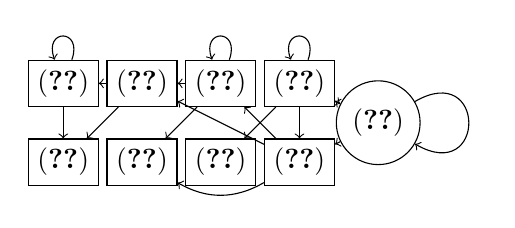
\begin{tikzpicture}
            \node[shape=rectangle,draw=black!100] (A) at (0,1) {\eqref{R-div-adp-1}};
            \node[shape=rectangle,draw=black!100] (B) at (0,0) {\eqref{R-div-adp-2}};
            \node[shape=rectangle,draw=black!100] (C) at (1,0) {\eqref{R-div-adp-3}};
            \node[shape=rectangle,draw=black!100] (D) at (2,0) {\eqref{R-div-adp-4}};
            \node[shape=rectangle,draw=black!100] (E) at (2,1) {\eqref{R-div-adp-5}};
            \node[shape=rectangle,draw=black!100] (F) at (1,1) {\eqref{R-div-adp-6}};
            \node[shape=rectangle,draw=black!100] (G) at (3,1) {\eqref{R-div-adp-7}};
            \node[shape=rectangle,draw=black!100] (H) at (3,0) {\eqref{R-div-adp-8}};
            \node[shape=circle,draw=black!100] (I) at (4,0.5) {\eqref{B-com-adp-2}};
        
            \path [->,in=110,out=70,looseness=5] (A) edge (A);
            \path [->] (A) edge (B);
            \path [->] (F) edge (A);
            \path [->] (F) edge (B);
            \path [->,in=110,out=70,looseness=5] (E) edge (E);
            \path [->] (E) edge (C);
            \path [->] (E) edge (F);
            \path [->,in=110,out=70,looseness=5] (G) edge (G);
            \path [->] (G) edge (D);
            \path [->] (G) edge (H);
            \path [->] (G) edge (I);
            \path [->,in=330,out=210,looseness=1] (H) edge (C);
            \path [->] (H) edge (E);
            \path [->] (H) edge (F);
            \path [->,in=330,out=30,looseness=5] (I) edge (I);
            \path [->] (I) edge (G);
            \path [->] (I) edge (H);
        \end{tikzpicture}
  \end{wrapfigure}

\vspace*{-.8cm}
\begin{example}\label{ex:rel-dependency-graph}
    The dependency graph for the ADP problem $(\ADPairMain{\R_{\tdivl}},
    \ADPairBase{\R^{=}_{\tset 2}})$
    from \Cref{ADP-Divl} is shown on the right. 
    Here, nodes from $\ADPairMain{\R_{\tdivl}}$ are denoted by rectangles and the
    node from $\ADPairBase{\R^{=}_{\tset 2}}$ is a circle.
\end{example}

To detect possible ordinary infinite rewrite sequences as in \Cref{example:ordinary-infinite},
we again have to regard SCCs of the dependency graph,
where we only need to consider SCCs that contain a node from $\C{P}$,
because otherwise, all steps in the SCC are relative.
However, in the relative ADP framework,
non-termination can also be due to chains representing redex-creating sequences.
Here,
it does not suffice to
look at SCCs.
Thus, the relative dependency graph processor differs substantially from the corresponding
processor for ordinary rewriting (and also from the corresponding processor for the
probabilistic ADP framework in \cite{FLOPS2024}). 

\begin{example}[Dependency Graph for Redex-Creating TRSs]\label{ex:DepGraphRedexCreating}
    For $\R_2$ and $\R_2^=$ from \Cref{example:redex-creating},
    the dependency graph for  $(\ADPairMain{\R_2}, \ADPairBase{\R_2^{=}})$ from
    \Cref{ex:ADPs-for-redex-creation-1} can be \pagebreak[2] seen on the

    \noindent
    \begin{minipage}[t]{9cm}
        right.
        Here, we cannot regard the SCC $\{\tf \to \tc(\tF,\tA)\}$ separately,
        as we need the rule  $\ta \to \tb$ from $\ADPairMain{\R_2}$ \linebreak
    \end{minipage}
    \hspace*{0.05cm}
    \begin{minipage}[t]{2.5cm}
        \begin{center}
            \scriptsize
            \vspace*{-0.4cm}
            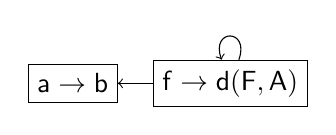
\begin{tikzpicture}
                \node[shape=rectangle,draw=black!100] (A) at (0,0) {$\ta \to \tb$};
                \node[shape=rectangle,draw=black!100] (B) at (2,0) {$\tf \to \tc(\tF,\tA)$};
            
                \path [->,in=110,out=70,looseness=5] (B) edge (B);
                \path [->] (B) edge (A);
            \end{tikzpicture}
        \end{center}
    \end{minipage}

    \vspace*{-0.3cm}
    \noindent
    to reduce the created redex.
    To find the ADPs that can reduce the created redexes,
    we have to regard the outgoing paths
    from the SCCs of $\C{P}^=$  to ADPs of $\C{P}$. 
\end{example}

The structure that we are looking for in the redex-creating case is 
 a path from an SCC to a node from $\C{P}$
 (i.e., a form of a \emph{lasso}),
which is \emph{minimal} in the sense that if we reach a node from $\C{P}$, then we stop
and do not move further along the edges of the graph.
Moreover, the SCC needs to contain an ADP with more than one annotated symbol, as otherwise the
generation of the infinitely many
$\C{P}$-redexes would not be possible.
Here, it suffices to look at SCCs in the graph restricted to only $\C{P}^{=}$-nodes (i.e.,
to SCCs in the $(\flat(\C{P}),\C{P}^{=})$-dependency graph).
The reason is that
if the SCC contains a node from $\C{P}$, then as mentioned above,
we have to prove anyway
that the SCC does not give rise to infinite chains.


\begin{definition}[$\mathtt{SCC}^{(\C{P},\C{P}^{=})}_{\C{P}'}$, $\mathtt{Lasso}$]\label{def:lasso}
    Let $(\C{P},\C{P}^{=})$ be an ADP problem.
    For any $\C{P}' \subseteq \C{P} \cup \C{P}^{=}$,
    let $\mathtt{SCC}^{(\C{P},\C{P}^{=})}_{\C{P}'}$ denote 
    the set of all SCCs of the
    $(\C{P},\C{P}^{=})$-dependency graph that contain an ADP from
    $\C{P}'$. Moreover, let  $\C{P}^{=}_{>1} \subseteq \C{P}^{=}$ denote the set of all
    ADPs from $\C{P}^{=}$ with
    more than one annotation.
    Then the set of all \defemph{minimal lassos} is defined as
    $\mathtt{Lasso} = \{\QQ \cup \{n_1, \ldots, n_k\} \mid \QQ \in
    \mathtt{SCC}^{(\flat(\C{P}),\C{P}^{=})}_{\C{P}^{=}_{>1}}, \; n_1,\ldots,n_k$ is a path such that $n_1 \in \QQ, \; n_k \in \C{P}, \text{ and } n_i \not\in \C{P} \text{ for all } 1 \leq i \leq k-1\}$.
\end{definition}

We remove the annotations of ADPs which do not have to be considered anymore\linebreak for
$\mathbf{p}$-steps due to the dependency graph, 
but we keep the ADPs for possible $\mathbf{r}$-steps and thus, consider
them as relative (base) ADPs.

\begin{restatable}[Dep.\ Graph Processor]{theorem}{RelativeDepGraphProc}\label{theorem:rel-DGP}
    Let $(\C{P},\C{P}^{=})$ be an ADP problem.
    Then

    \vspace*{-.4cm}
    
    {\small\begin{align*}
        \Proc_{\mathtt{DG}}(\C{P},\C{P}^{=}) & =
        \{ (\,\C{P} \cap \QQ, \;
        (\C{P}^= \cap \QQ)\cup        \flat( \,(\C{P} \cup \C{P}^{=}) \setminus \QQ \,)\,
           )
        \mid \QQ
        \in \mathtt{SCC}_{\C{P}}^{(\C{P}, \C{P}^{=})} \cup \mathtt{Lasso}\} \! 
    \end{align*}
    }

    \vspace*{-.1cm}

    \noindent
    is sound and complete.   
\end{restatable}

\begin{example}\label{ex:DivlDepGraph}
    For $(\ADPairMain{\R_{\tdivl}}, \ADPairBase{\R^{=}_{\tset 2}})$ from
    \Cref{ex:rel-dependency-graph} we have three SCCs 
    $\{\eqref{R-div-adp-1}\}$, $\{\eqref{R-div-adp-5}\}$, 
    and $\{\eqref{R-div-adp-7},\eqref{B-com-adp-2}\}$ containing nodes from $\ADPairMain{\R_{\tdivl}}$.
    The set $\{\eqref{B-com-adp-2}\}$ is the only
    SCC of $(\flat(\ADPairMain{\R_{\tdivl}}), \ADPairBase{\R^{=}_{\tset 2}})$ and there
    are paths from that SCC to the ADPs $\eqref{R-div-adp-7}$ and
    $\eqref{R-div-adp-8}$ of $\C{P}$. However, they are not in
    $\mathtt{Lasso}$, because the SCC $\{\eqref{B-com-adp-2}\}$ does not contain an ADP with more than one
    annotation.
    Hence, we result in the three new ADP problems 
    $(\{\eqref{R-div-adp-1}\} \cup \flat(\ADPairMain{\R_{\tdivl}} \setminus \{\eqref{R-div-adp-1}\}), \{\flat(\ref{B-com-adp-2})\})$,
    $(\{\eqref{R-div-adp-5}\} \cup \flat(\ADPairMain{\R_{\tdivl}} \setminus \{\eqref{R-div-adp-5}\}), \{\flat(\ref{B-com-adp-2})\})$,
    and 
    $(\{\eqref{R-div-adp-7}\} \cup \flat(\ADPairMain{\R_{\tdivl}} \setminus \{\eqref{R-div-adp-7}\}),\{(\ref{B-com-adp-2})\})$.
    For the first two of these new ADP problems, 
    we can use the derelatifying processor of \Cref{theorem:derel-proc-1} and prove SN via ordinary DPs, since their base
    ADP $\flat(\ref{B-com-adp-2})$ does not contain any annotated symbols anymore.
\end{example}

The dependency graph processor in combination with the derelatifying processors of \Cref{theorem:derel-proc-1,theorem:derel-proc-2}
already subsumes the techniques of
\Cref{theorem:main-relative-rewrite-corollary-yamada-1,theorem:main-relative-rewrite-corollary-yamada-2}.
The reason is that if $\R$ dominates $\R^{=}$, then there is no edge from an ADP of $\ADPairBase{\R^{=}}$ to
any ADP of $\ADPairMain{\R}$ in the $(\ADPairMain{\R}, \ADPairBase{\R^{=}})$-dependency
graph. Hence, there are no minimal lassos and the
dependency graph processor just creates ADP problems from the SCCs of $\ADPairMain{\R}$
where the base ADPs do not have any annotations anymore. Then \Cref{theorem:derel-proc-1}
allows us to switch to ordinary DPs.
For example, if we consider $\R^{=}_{\tset}$ instead of $\R^{=}_{\tset 2}$, then the
dependency graph processor \pagebreak[2]  only yields the two subproblems for the SCCs 
$\{\eqref{R-div-adp-1}\}$ and $\{\eqref{R-div-adp-5}\}$, 
where the base ADPs do not\linebreak contain any annotations anymore.
Then, we can move to ordinary
DPs via \Cref{theorem:derel-proc-1}.

Compared to
\Cref{theorem:main-relative-rewrite-corollary-yamada-1,theorem:main-relative-rewrite-corollary-yamada-2},
the dependency graph allows for more precise
over-approximations than just ``dominance'' in order
to detect when the base ADPs do not depend on 
the main ADPs.  Moreover,
the derelatifying processors of \Cref{theorem:derel-proc-1,theorem:derel-proc-2}
allow us to switch to  the ordinary DP framework also for subproblems which result 
from the application of other processors of our relative ADP framework.
In other words, \Cref{theorem:derel-proc-1,theorem:derel-proc-2} allow us to apply this
switch in a modular way, even if their prerequisites
do not hold for the initial canonical ADP problem (i.e., even if the prerequisites of \Cref{theorem:main-relative-rewrite-corollary-yamada-1,theorem:main-relative-rewrite-corollary-yamada-2}
do not hold for the whole TRSs).


\subsection{Relative Reduction Pair Processor}\label{Relative Reduction Pair Processor}

Next, we adapt the reduction pair processor to ADPs for relative rewriting.
While the reduction pair processor for ADPs in the probabilistic setting
\cite{FLOPS2024} was restricted to polynomial interpretations,
we now allow arbitrary
reduction pairs
using a similar idea as in 
the reduction pair processor from \cite{noschinski2013analyzing} for complexity analysis
via dependency tuples.

To find out which ADPs cannot be used for infinitely many $\mathbf{p}$-steps,
the idea is not to compare the annotated left-hand side with the
whole right-hand side, but just with the set of its annotated subterms.
To combine these subterms in the case of
ADPs with two or no annotated symbols, we extend the signature by two fresh \emph{compound} symbols
$\Com{0}$ and $\Com{2}$ of arity $0$ and $2$, respectively.
Similar to \cite{noschinski2013analyzing},
we have to use $\Com{}$\emph{-monotonic} and $\Com{}$\emph{-invariant} reduction pairs.

\begin{definition}[$\Com{}$-Monotonic, $\Com{}$-Invariant]\label{def:poly-interpretation-for-depset}
    For $r \in \TSet{\SignatureADC}{\VSet}$, we define
    $\subA(r) = \Com{0}$ if $r$ does not contain any annotation,
    $\subA(r) = t^\#$ if $t \trianglelefteq_{\#} r$ and $r$ only contains one annotated symbol,
    and $\subA(r) = \Com{2}(r_1^\#, r_2^\#)$ if $r_1 \trianglelefteq_{\#}^{\pi_1} r$,
    $r_2 \trianglelefteq_{\#}^{\pi_2} r$, 
    and $\pi_1 <_{lex} \pi_2$ where $<_{lex}$ is the (total)
    lexicographic order on positions.

    A reduction pair $(\succsim, \succ)$ is called \defemph{$\Com{}$-monotonic}
    if $\Com{2}(s_1, t) \succ
    \Com{2}(s_2, t)$ and $\Com{2}(t, s_1) \succ
    \Com{2}(t, s_2)$ for all $s_1,s_2,t \in \TSet{\SignatureADC}{\VSet}$ with $s_1 \succ s_2$.
    Moreover, it is  \defemph{$\Com{}$-invariant}
    if $\Com{2}(x,y) \sim \Com{2}(y,x)$ and
    $\Com{2}(x,\Com{2}(y,z)) \sim 
    \Com{2}(\Com{2}(x,y),z)$
    for ${\sim} = {\succsim} \cap {\precsim}$. 
\end{definition}
So for example, reduction pairs based on polynomial interpretations are
$\Com{}$-monotonic and $\Com{}$-invariant if $\Com{2}(x,y)$ is interpreted by $x + y$.

For an ADP problem $(\C{P},\C{P}^{=})$, 
now the reduction pair processor has to orient the non-annotated rules $\flat(\C{P} \cup
\C{P}^{=})$ weakly and for all ADPs $\ell \to r$,
it compares the annotated left-hand side  $\ell^\#$ with
$\subA(r)$. In strictly decreasing ADPs, one can then remove all annotations and consider
them as relative (base) ADPs again.

\begin{restatable}[Reduction Pair Processor]{theorem}{RelRPP}\label{thm:RelRPP}
    Let $(\C{P},\C{P}^{=})$ be an ADP problem and let
    $(\succsim, \succ)$ be a $\Com{}$-monotonic and $\Com{}$-invariant reduction pair
    such that $\flat(\C{P} \cup \C{P}^{=})\linebreak \subseteq {\succsim}$ and
    $\ell^\# \succsim \subA(r)$ for all $\ell \to r \in \C{P} \cup \C{P}^{=}$.
    Moreover, let $\PP_{\succ} \subseteq \C{P} \cup \C{P}^{=}$ 
    such that\linebreak $\ell^\# \succ \subA(r)$ for all $\ell \to r \in \PP_{\succ}$. 
    Then $\Proc_{\mathtt{RPP}}(\C{P},\C{P}^{=}) = \{(\C{P} \setminus \PP_{\succ}, (\C{P}^{=} \setminus \PP_{\succ}) \cup
    \flat(\PP_{\succ}))\}$ is sound and complete.
\end{restatable}

\begin{example}\label{example:rel-RPP}
    For the remaining ADP problem
    $(\{\eqref{R-div-adp-7}\} \cup \flat(\ADPairMain{\R_{\tdivl}} \setminus \{\eqref{R-div-adp-7}\}),\{(\ref{B-com-adp-2})\})$ 
    from \Cref{ex:DivlDepGraph}, we can apply the reduction pair processor
    using the polynomial interpretation from the end of \Cref{Dependency Pairs for Ordinary Term Rewriting} which maps 
    $\O$ to $0$, $\ts(x)$ to $x + 1$,
    $\tcons(y,\xs)$ to $\xs + 1$, $\tDL(x,\xs)$ to $\xs$,
    and all other symbols to their first arguments. 
    Then, $\eqref{R-div-adp-7}$ is oriented strictly (i.e., it is in
    $\PP_{\succ}$) and $\eqref{B-com-adp-2}$ is oriented weakly.
    Hence, we remove the annotation from $\eqref{R-div-adp-7}$ and move it to the base
    ADPs.
    Now there is no SCC with a main ADP anymore in the
    dependency graph, and thus the dependency graph processor 
    returns $\emptyset$.
    This proves SN for $(\ADPairMain{\R_{\tdivl}}, \ADPairBase{\R^{=}_{\tset 2}})$, hence
    $\R_{\tdivl} / \R^{=}_{\tset 2}$ is also SN.
\end{example}

\begin{example}\label{ex:RPPCreating}
    Regard the ADPs
    $\ta \to \tb$  and $\tf \to \tc(\tF,\tA)$ for
    the redex-creating  \Cref{example:redex-creating} again.
    When using  a polynomial interpretation  $\mathrm{Pol}$ that maps $\Com{0}$ to $0$ and
    $\Com{2}(x,y)$ to $x + y$, then for the reduction pair processor 
    one has to satisfy $\mathrm{Pol}(\tA) \geq 0$ and
    $\mathrm{Pol}(\tF) \geq \mathrm{Pol}(\tF) + \mathrm{Pol}(\tA)$, i.e.,
    one cannot
    make any of the ADPs strictly decreasing.

    In contrast, for the variant
    with the terminating base rule  $\tf(\ts(y)) \to \tc(\tf(y),\ta)$ from \Cref{terminatingRedexDuplCreate},
    we have the ADPs $\ta \to \tb$  and $\tf(\ts(y)) \to \tc(\tF(y),\tA)$. 
    Here, the second constraint is  $\mathrm{Pol}(\tF(\ts(y))) \geq
    \mathrm{Pol}(\tF(y)) + \mathrm{Pol}(\tA)$. To make 
    one of the ADPs strictly decreasing,
    one can set
    $\mathrm{Pol}(\tF(x)) = x$, $\mathrm{Pol}(\ts(x)) = x+1$, and
    $\mathrm{Pol}(\tA) = 1$ or $\mathrm{Pol}(\tA) = 0$.
    Then the reduction pair processor
    removes the annotations from the strictly decreasing ADP and 
     the dependency graph processor  proves SN.
\end{example}

\section{Evaluation and Conclusion}\label{Evaluation and Conclusion}

In this paper, we introduced the first
notion of (annotated) dependency pairs
and the first DP framework
for relative termination, which also features suitable
dependency graph and reduction pair processors for relative ADPs.
Of course, 
further classical DP processors can be adapted to our relative ADP framework as well. For
example, in our implementation of the novel ADP framework in our tool \aprove{} \cite{JAR-AProVE2017},
we also included a
straightforward adaption of the classical \emph{rule removal processor}
\cite{gieslLPAR04dpframework}, see 
\Cref{Appendix}.\footnote{This processor works
analogously to the preprocessing
at the beginning
of \Cref{Relative DP Framework}
which can be used to remove duplicating rules: For an  ADP problem $(\C{P},\C{P}^{=})$, it tries to find
a reduction pair 
$(\succsim, \succ)$ 
where $\succ$ is closed under contexts
such that $\flat(\C{P} \cup \C{P}^{=}) \subseteq {\succsim}$.
Then for $\PP_{\succ} \subseteq \C{P} \cup \C{P}^{=}$ 
with $\flat(\C{P}_{\succ}) \subseteq {\succ}$, the processor replaces the ADP by 
$(\C{P} \setminus \PP_{\succ}, \C{P}^{=} \setminus \PP_{\succ})$.}
In future work, we will investigate how to use our new form of 
ADPs for full (instead of innermost) rewriting also in the probabilistic setting 
and for complexity analysis.



To evaluate the new relative ADP framework, we compared its implementation in 
``\emph{new} \aprove{}'' 
to all other tools that participated
in the most recent \emph{termination competition (TermComp 2023)} \cite{termcomp}
on relative rewriting, i.e.,
\natt{} \cite{natt_sys_2014},  \ttttwo{} \cite{ttt2_sys}, \mnm{} \cite{FSCD19}, and ``\emph{old} \aprove{}'' which did
not yet contain the contributions of the current paper.
In \emph{TermComp 2023}, 
98 benchmarks were used for relative termination. However, these benchmarks only consist
of
examples where the main TRS
$\R$ dominates the base TRS $\R^{=}$ (i.e., which can be handled by \Cref{theorem:main-relative-rewrite-corollary-yamada-1} from
\cite{iborra2017relative})
or which can already
be solved via simplification orders directly.
Therefore, we extended the collection by
17 new examples,
including both
$\R_{\tdivl}/\R^{=}_{\tset}$ from \Cref{ex:divlTRS,ex:mset1},
and our leading example $\R_{\tdivl} / \R^{=}_{\tset 2}$ 
from \Cref{ex:mainExample} (where only \emph{new} \aprove{} can prove SN).
Except for $\R_{\tdivl}/\R^{=}_{\tset}$, in these examples
$\R$ does not dominate $\R^{=}$. 
Most of these examples adapt well-known classical TRSs from the
\emph{Termination Problem Data Base} \cite{tpdb} used at \emph{TermComp}
to the relative setting.
In the following table,
the number in the ``YES'' (``NO'') row indicates for how many of the 115
examples the respective
tool could prove (disprove) relative termination and ``MAYBE'' refers to the benchmarks
where the tool could not solve the problem within the timeout of 300~s per example. The numbers in
brackets are the respective results when only considering our new 17 examples.
``AVG(s)'' gives the average runtime of the tool
on solved examples in seconds.

\begin{center}
{\small    \begin{tabular}{||c | c | c | c | c | c||}
     \hline
      & \emph{new} \aprove & \natt & \emph{old} \aprove & \ttttwo & \mnm  \\ [0.5ex] 
     \hline
     YES & 78 (17) & 65 (7) & 47 (4) & 39 (3) & 0 (0)  \\ 
     \hline
     NO & 13 (0)& 5 (0)& 13 (0)& 7 (0)& 13 (0)\\ 
     \hline
     MAYBE & 24 (0)& 45 (10)& 55 (13)& 69 (14) & 102 (17) \\ 
     \hline
      AVG(s) & 6.68 & 0.38 & 3.67 & 1.61 & 1.28  \\ 
     \hline
    \end{tabular}}
\end{center}



The table clearly shows that while \emph{old} \aprove{} was already the second most powerful
tool for relative termination, the integration of the ADP framework in \emph{new} \aprove{}
yields a substantial advance in power (i.e., it only fails on 24 of the examples, compared
to 45 and 55 failures of \natt{} and \emph{old} \aprove, respectively).
In particular,  previous tools (including 
\emph{old} \aprove{}) often have problems with
relative TRSs where the main TRS does
 not dominate the base TRS, whereas the ADP framework can handle
 such examples.


A special form of relative TRSs are \emph{relative string rewrite systems (SRSs)}, where all function
symbols have arity 1.
Due to the base ADPs with two annotated
symbols on the right-hand side, 
here the ADP framework is less powerful
than dedicated techniques for string rewriting.
For the 403 relative SRSs at \emph{TermComp 2023},
the ADP framework only finds 71 proofs, mostly due to the dependency graph and the rule removal processor, 
while termination analysis via \aprove's
standard strategy for relative SRSs
succeeds on 209 examples, and the two most powerful tools for relative SRSs at
\emph{TermComp 2023} (\mnm{} and \matchbox{} \cite{matchbox})
succeed on 274 and 269 examples, respectively.


Another special form of relative rewriting is \emph{equational rewriting}, where one has
a set of equations $E$ which correspond to relative rules that can be applied in both directions.
In \cite{RTA01}, DPs were adapted to equational rewriting.
However, this approach requires
$E$-unification to be decidable and finitary
(i.e., for (certain) pairs of terms, 
it has to compute  finite complete sets of $E$-unifiers).
This works well if $E$
are AC- or C-axioms, and for this special case, dedicated techniques like
\cite{RTA01} are more powerful than our new ADP framework for relative termination.
For example, on the 76 AC- and C-benchmarks  for equational rewriting at \emph{TermComp 2023},
the  relative ADP framework  finds 36 proofs, while dedicated
tools for AC-rewriting like \aprove's equational strategy or \muterm{} \cite{gutierrez_mu-term_2020} succeed on
66 and 64 examples, respectively.
However, in general, the requirement of a finitary
$E$-unification algorithm is a  hard restriction.
In contrast to existing tools for equational rewriting,
our new ADP framework can be used for arbitrary
(non-duplicating) relative rules.

For details on our experiments, our collection of examples,
and for instructions on how to run our implementation
in \textsf{AProVE} via its \emph{web interface} or locally, see
\url{https://aprove-developers.github.io/RelativeDTFramework/}


\paper{\printbibliography}
\report{\bibliographystyle{splncs04}
 %\bibliography{biblio}
 \documentclass[12pt]{article}

\begin{document}
    \section{First section}
        \subsection{First subsection}
            Content of the first subsection.

        \subsection{Second subsection}
            Another piece of content of the second subsection.
            \begin{itemize}
                \item First item in the second subsection.
                \item Second item.
                \item Third and last item.
            \end{itemize}

        \subsection{Third subsection}
            Third subsection's content.

\end{document}
}


\report{
  \clearpage

\appendix
%!TEX root = ./paper.tex 

\section{Sum of $k$ Laplace variables} % (fold)
\label{app:laplace}

Consider the random variable $Y_k = \sum_{i=1}^k X_i/\sqrt{2k}$ where the $X_i$ variables have a Laplace distribution with density
\begin{equation}\label{eq:laplace}
p(x) = \frac{1}{2}\exp(-\abs{x}).
\end{equation}

It is easy to see that this variable is centred and has unit variance, as $\mathbb{E}\left[Y_k\right]=\sqrt{k}\mathbb{E}\left[X_i\right]=0$ and $\mathbb{E}\left[Y_k^2\right]= \frac{\mathbb{E}\left[X_i^2\right]}{2}=1$.

To compute the density of $Y_k$ we will compute its characteristic function $\mathbb{E}\left[\exp\left(\iu t Y_k\right)\right]$, which is none other than the Fourier transform of its density. It can be computed in terms of the characteristic function of the Laplace random variables, obtained by a Fourier transform on the expression in Eq~\eqref{eq:laplace}, as:

\begin{equation}\label{eq:characteristic_function}
\phi_X(t)= \frac{1}{2} \int \dint x~ e^{\iu tx - \abs{x}}= \frac{1}{1+t^2}.
\end{equation}

The characteristic function of $Y_k$ can then be easily written using this function, 
\begin{equation}\label{eq:characteristic_Y}
\phi_{Y_k}(t) = \left[\phi_X\left(\frac{t}{2k}\right)\right]^k = \frac{2^k k^k}{\left(2k+t^2\right)^k}.
\end{equation}

To find the density it is therefore only necessary to invert this transformation.

\subsection{Computing the density for $Y_k$} % (fold)
\label{sub:computing_the_density_for_}

To find the density of $Y_k$, $g_k(y)$, we compute the inverse Fourier transform of its characteristic function, i.e.:

\begin{equation}\label{eq:fourier_inv}
\begin{split}
g_k(y) &=\frac{2^kk^k}{2 \pi} \int \dint t~ \frac{e^{-\iu t y}}{\left(2k+t^2\right)^k}\\
&=\frac{2^kk^k}{2\pi} \int_{\mathcal{C}} \dint z~ f(z)
\end{split}
\end{equation}
with $f(z)=\frac{e^{-\iu z y}}{\left(2k+z^2\right)^k}=\frac{e^{-\iu z y}}{\left(z-\iu\sqrt{2k}\right)^k \left(z+\iu\sqrt{2k}\right)^k}$.

This computation can be done via a complex-plane integral along a contour $\mathcal{C}$ running from $-R$ to $R$ and then around the half-circle centred at the origin and of radius $R>\sqrt{2k}$. The contour is chosen so that it encloses $-\iu\sqrt{2k}$ if $y>0$ and $\iu\sqrt{2k}$ if $y<0$, and then the limit $R\to\infty$ is taken. See Figure~\ref{fig:contour} for an illustration for $y>0$.

\begin{figure}[tb]
    \centering
    \includegraphics[width=8cm]{figures/semicircle.pdf}
    \caption{Example of the contour taken in the case $y>0$.}
    \label{fig:contour}
\end{figure}

In this case, the function $f(z)$ has a pole of order $k$ at $z=-\iu$, of residue

\begin{equation}\label{eq:residue_1}
\mbox{Res}_{-\iu\sqrt{2k}}(f) = \frac{1}{(k-1)!}\lim_{z\to -\iu\sqrt{2k}} \frac{\partial^{(k-1)}}{\partial z^{(k-1)}}\left(\frac{e^{-\iu z y}}{\left(z-\iu\sqrt{2k}\right)^k }\right). 
\end{equation}


To compute the derivative, we apply the generalized Leibniz' rule:
\begin{equation}\label{eq:leib_rule}
\frac{\partial^{(k-1)}}{\partial z^{(k-1)}}\left(\frac{e^{-\iu z y}}{\left(z-\iu\sqrt{2k}\right)^k }\right)= \sum_{l=0}^{k-1}\binom{k-1}{l}\frac{\partial^l}{\partial z^l}\left(e^{-\iu z y}\right)\frac{\partial^{(k-1-l)}}{\partial z^{(k-1-l)}} \left((z-\iu\sqrt{2k})^{-k}\right),
\end{equation}
which then allows for an explicit computation of the residue in Eq.~\eqref{eq:residue_1}:
\begin{equation}\label{eq:full_residue}
\mbox{Res}_{-\iu}(f)= \iu\frac{1}{\left(k-1\right)!}\sum_{l=0}^{k-1}\binom{k-1}{l} \left(2\sqrt{2k}\right)^{l+1-2k} \frac{(2k-2-l)!}{(k-1)!} y^l e^{-\sqrt{2k}y}.
\end{equation}

Plugging this into $g_k(y)=\frac{(2k)^k}{2\pi}\int_{\mathcal{C}}f=-\iu (2k)^k \mbox{Res}_{-\iu}(f)$, and considering the symmetrical case when $y<0$, we obtain
\begin{equation}\label{eq:full_result}
\begin{split}
g_k(y) &= \frac{2^{-2k}2\sqrt{2k}}{\left(k-1\right)!}\sum_{l=0}^{k-1}\binom{k-1}{l} 2^l \frac{(2k-2-l)!}{(k-1)!} (\sqrt{2k}\abs{y})^l e^{-\sqrt{2k}\abs{y}}.
\end{split}
\end{equation}

One can then check how this behaves on Figure~\ref{fig:lap_sum}, where it is evident that the Laplace cusp is not stable upon aggregation of variables. 

\begin{figure}[tb]
    \centering
    \includegraphics[width=.8\textwidth]{figures/fig_laplace_sum.pdf}
    \caption{Examples of the sum of $k$ Laplace variables for $k=\{1,2,4,8\}$ with a Gaussian for comparison. Note that the Laplace ``cusp'' is already gone at $k=2$.}
    \label{fig:lap_sum}
\end{figure}

\subsection{Extension to sums of correlated Laplace variables} % (fold)
\label{sub:extension_to_sums_of_correlated_laplace_variables}
Suppose now that we want to compute the distribution of the sum of two Laplace random variables $X_1$ and $X_2$, with $\mathbb{E}(X_1X_2)=\rho$, and where both variables have the density given in Eq.~\eqref{eq:laplace}.

To tackle this problem, we first prove a preliminary result, which is that the variables $X$ can be represented as a superposition of Gaussian random variables with variances distributed according to an exponential distribution, namely

\begin{equation}\label{eq:lap_super}
X \overset{\text{law}}{=} \mathbb{E}_{\sigma}\left[Y_{\sigma}\right] ,
\end{equation}
where the distribution of $Y_{\sigma}$ and of $\sigma$\footnote{Mind that $\sigma$ is the square root of the variance, and that it is only its square that is distributed exponentially.} are given by

\begin{equation}\label{eq:densities}
p_{Y_{\sigma}}(y) = \frac{1}{\sqrt{2\pi\sigma^2}} e^{-y^2/2\sigma^2},\quad p_{\sigma}(\sigma)= \sigma e^{-\sigma^2/2}\mathbf{1}_{\sigma>0}.
\end{equation}

To prove this, one need only compute the characteristic function of $X$ as
\begin{equation}\label{eq:characteristic_function_superp}
\begin{split}
\phi_{X}(t) &= \int_{0}^\infty\dint \sigma ~ \sigma e^{-\sigma^2/2}\left[\int \frac{\dint y}{\sqrt{2\pi \sigma^2}}\exp\left(-\frac{y^2}{2\sigma^2}+ity\right)\right]\\
&=\int_{0}^\infty\dint \sigma~ \sigma \exp\left(-\frac{\sigma^2}{2}\left(1+t^2\right)\right)\\
&= \frac{1}{1+t^2},
\end{split}
\end{equation}
which proves our assertion.

We can now generalize to try to find the sum of $k$ correlated Laplace variables. To do this, we will consider the sum $\sum_{l=1}^{k}\sigma_l Y_l$ where $Y_0$ is Gaussian and
\begin{equation}\label{eq:ar1}
Y_{l} = \rho Y_{l-1} + \sqrt{1-\rho^2} \eta_l, 
\end{equation}
with $\eta_l$ a Gaussian white noise of unit variance and $\sigma_l$ distributed according to the density in Eq.~\eqref{eq:densities}. One sees that in this case the variables $\sigma_l Y_l$ are Laplace-distributed, with $\Cor(\sigma_l Y_l, \sigma_{l+1}Y_{l+1})=2\rho $. 

For $k=2$ the sum is 
\begin{equation}\label{eq:s2}
 S_2 = \sigma_1Y_1 + \sigma_2 Y_2 = \sigma_1 Y_1 + \rho \sigma_2 Y_1 + \sigma_2 \sqrt{1-\rho^2}\eta_2,
 \end{equation} 
 which, owing to the Gaussian nature of $Y_1,Y_2$ and $\eta_2$ can be written as
 \begin{equation}\label{eq:rewriting}
 S_2 = \sqrt{\left(\sigma_1 + \rho\sigma_2\right)^2 + \sigma_2^2 \left(1-\rho^2\right)}\xi,
 \end{equation}
 with $\xi$ Gaussian with unit variance. 

 We can then compute the characteristic function of $S_2$ given $(\sigma_1,\sigma_2)$:

\begin{equation}
    \phi_2(t,\sigma_1,\sigma_2)=\mathbb{E}\left[\exp\left(\iu t S_2\right) |\sigma_1, \sigma_2\right] = \exp\left(-\frac{\left(\sigma_1 + \rho\sigma_2\right)^2 + \sigma_2^2 \left(1-\rho^2\right)}{2}t^2\right).
\end{equation}


This last expression can then be averaged using the distributions of $\sigma_1$ and $\sigma_2$ to obtain the characteristic function of $S_2$:

\begin{equation}\label{eq:nasty_int}
\begin{split}
\phi_2(t) &= \int_{0}^{\infty}\dint \sigma_1~\sigma_1e^{-\frac{\sigma_1^2}{2}}\int_{0}^{\infty}\dint \sigma_2~\sigma_2e^{-\frac{\sigma_2^2}{2}}\phi_2(t,\sigma_1,\sigma_2)\\
&= \int_{0}^{\infty}\dint \sigma_1 \int_{0}^{\infty}\dint \sigma_2~~\sigma_1\sigma_2 \exp\left(-\frac{1}{2}\Braket{\sigma | \mathbf{A} | \sigma}\right),
\end{split}
\end{equation}
where the matrix $\mathbf{A}= \left( \begin{matrix}
1+t^2 & t^2\rho \\ t^2\rho & 1+t^2
\end{matrix}  \right)$ has two eigenvectors, $\ket{u} = \frac{1}{\sqrt{2}}\left(1,1\right)$ corresponding to eigenvalue $\lambda_1 = 1+t^2\left(1-\rho\right)$  and $\ket{v}=\frac{1}{\sqrt{2}}(1,-1)$ corresponding to  $\lambda_2 = 1+t^2\left(1+\rho\right)$. The dependence in $t$ of $\lambda_1,\lambda_2$ is implicit.


Next, we substitute $u=\frac{\sqrt{2}}{2}\left(\sigma_1+\sigma_2\right)$ and $v=\frac{\sqrt{2}}{2}\left(\sigma_1-\sigma_2\right)$ in Eq.~\eqref{eq:nasty_int}, to obtain
\begin{equation}
\begin{split}
\phi_2(t) =& \frac{1}{2}\int\dint v \int \dint u ~\left(u^2-v^2\right)\exp\left(-\lambda_1\frac{u^2}{2}-\lambda_2\frac{v^2}{2}\right)\mathbf{1}_{u+v>0}\mathbf{1}_{u-v>0} \\
=& \frac{1}{2}\int\dint v \int \dint u~u^2 \exp\left(-\lambda_1\frac{u^2}{2}-\lambda_2\frac{v^2}{2}\right)\mathbf{1}_{u+v>0}\mathbf{1}_{u-v>0}\\
&+ \frac{1}{2}\int\dint v \int \dint u~v^2 \exp\left(-\lambda_1\frac{u^2}{2}-\lambda_2\frac{v^2}{2}\right)\mathbf{1}_{u+v>0}\mathbf{1}_{v-u>0}.
\end{split}
\end{equation}


This integral can be computed explicitly, first by integrating over $v$ and then by setting $w=\sqrt{\frac{\lambda 1}{2}}u$, to get
\begin{equation}\label{eq:nasty_1}
\begin{split}
\int \dint u~e^{-\lambda_1 \frac{u^2}{2}}u^2 \int\dint v~ e^{-\lambda_2 \frac{v^2 }{2}}\mathbf{1}_{u+v>0}\mathbf{1}_{u-v>0} &= 2\sqrt{\frac{\pi}{2\lambda_2}} \int_{0}^{\infty}\dint u~e^{-\lambda_1 \frac{u^2}{2}}u^2 \text{erfc}\left(\sqrt{\frac{\lambda_2}{2}}u\right)\\
&= 4\sqrt{\frac{\pi}{\lambda_2}}\frac{1}{\lambda_1^{3/2}}\int_{0}^{\infty}\dint w~e^{-w^2}w^2 \text{erfc}\left(\sqrt{\frac{\lambda_2}{\lambda_1} w} \right),
\end{split}
\end{equation}
with the last integral giving (see e.g. \cite{Ng_Geller_1969})
\begin{equation}
    \int_{0}^{\infty}\dint w~e^{-w^2}w^2 \text{erfc}\left(\sqrt{\frac{\lambda_2}{\lambda_1} w} \right) = \frac{1}{2\sqrt{\pi}}\left(\arctan\left(\sqrt{\frac{\lambda_1}{\lambda_2}}\right)- \frac{\lambda_1}{\lambda_2+\lambda_1}\sqrt{\frac{\lambda_2}{\lambda_1}}\right).
\end{equation}


Plugging this last expression back into Eq.~\eqref{eq:nasty_1} leads to
\begin{equation}\label{eq:nasty_1_complete}
\begin{split}
\int \dint u~e^{-\lambda_1 \frac{u^2}{2}}u^2 \int\dint v~ e^{-\lambda_2 \frac{v^2 }{2}}\mathbf{1}_{u+v>0}\mathbf{1}_{u-v>0}  &= \frac{2}{\lambda_1^{3/2}\lambda_2^{1/2}}\left(\arctan\left(\sqrt{\frac{\lambda_1}{\lambda_2}}\right)- \frac{\lambda_1}{\lambda_2+\lambda_1}\sqrt{\frac{\lambda_2}{\lambda_1}}\right),
\end{split}
\end{equation}
from which we can give the full expression of the characteristic function $\phi_2(t)$:
\begin{equation}\label{eq:nasty_2}
\phi_2(t)=\frac{\arctan(\sqrt{\lambda_1/\lambda_2})}{\lambda_1^{3/2}\lambda_2^{1/2}}+\frac{\arctan(\sqrt{\lambda_2/\lambda_1})}{\lambda_2^{3/2}\lambda_1^{1/2}}-\frac{1}{\sqrt{\lambda_1\lambda_2}\left(\lambda_1+\lambda_2\right)}\left(\sqrt{\frac{\lambda_2}{\lambda_1}}+\sqrt{\frac{\lambda_1}{\lambda_2}}\right).
\end{equation}


We next study the properties of $p_2(s)$, the distribution of $S_2$, which is but the inverse Fourier transform of $\phi_2$. 
Given that $\abs{\rho}<1$, we can write $\lambda_1(t) = \left(1+t^2\right)\left(1-\frac{t^2}{1+t^2}\rho\right)$ and $\lambda_2(t)=\left(1+t^2\right)\left(1+\frac{t^2}{1+t^2}\rho\right)$, and so the asymptotic behaviour $\phi_2(t)\underset{\abs{t}\gg 1}{\propto}(1+t^2)^{-2}$ is clear. When $\abs{\rho}=1$ however, we have e.g. $\lambda_1=1$ and $\lambda_2 = 1+2t^2$, and as a consequence $\phi_2(t)\sim t^{-3}$ for large $t$.

One can then look at the curvature of the distribution function $p_2(s)$ of the sum $S_2$ defined in Eq.~\eqref{eq:s2}, given by
\begin{equation}
    p_2''(0) = \int \dint t~t^2 \phi(t),
\end{equation}
and see that it behaves as $(1-\abs{\rho})^{-3/2}$. Since this quantity is finite for $\abs{\rho}<1$, it follows that the distribution of $p_2(s)$ cannot have a Laplace cusp at $s=0$, as it would correspond to an infinite curvature.


In general for the case of the sum of $N$ Laplace variables with the correlation structure given in Eq.~\eqref{eq:ar1} one can generalize Eq.~\eqref{eq:nasty_int} with a circulant matrix
\begin{equation}\label{eq:a_matrix}
\mathbf{A} = \left( \begin{matrix}
1+t^2& t^2\rho& \ldots &t^2\rho^{N-2} &t^2\rho^{N-1}\\
t^2\rho& 1+t^2& t^2\rho& &t^2\rho^{N-2}\\
\vdots& t^2\rho& 1+t^2& \ddots& \vdots\\
t^2\rho^{N-2}& & \ddots& \ddots& t^2\rho \\
t^2\rho^{N-1}& t^2\rho^{N-2}& & t^2\rho & 1+t^2
\end{matrix} \right),
\end{equation}
leading to similar, though more complicated, computations.
}
\end{document}



